% !BIB program = biber
\documentclass[doc]{apa6}

%\usepackage{apacite}
\usepackage[utf8]{inputenc}
\usepackage[american]{babel}
\usepackage{todonotes}
\usepackage{csquotes}
\usepackage[style=apa,sortcites=true,sorting=nyt,backend=biber]{biblatex}
\usepackage{adjustbox}
\DeclareLanguageMapping{american}{american-apa}
%\addbibresource{bibliography.bib}
%\addbibresource{zot3.bib}
\addbibresource{zot3_amy.bib}
\usepackage{boxedminipage}
\usepackage[toc,page]{appendix}

\newcommand{\given}{\, | \,}

\title{When extremists win: Cultural transmission via iterated learning when populations are heterogeneous}
\shorttitle{Heterogenous iterated learning}

\fiveauthors{\normalsize Danielle J. Navarro}{\normalsize Amy Perfors}{\normalsize Arthur Kary}{\normalsize Scott D. Brown}{\normalsize Chris Donkin}
\fiveaffiliations{School of Psychology\\University of New South Wales}{School of Psychology\\University of Melbourne}{School of Psychology\\University of New South Wales}{School of Psychology\\University of Newcastle}{School of Psychology\\University of New South Wales}

\abstract{How does the process of information transmission affect the cultural or linguistic products that emerge? This question is often studied experimentally and computationally via iterated learning: a procedure in which participants learn from previous participants in a chain. Iterated learning is a powerful tool because, when all participants share the same priors, the stationary distributions of the iterated learning chains reveal those priors. In many situations, however, it is unreasonable to assume that all participants share the same prior beliefs. We present four simulation studies and one experiment demonstrating that when the population of learners is heterogeneous, the behavior of an iterated learning chain can be unpredictable, and is often systematically distorted by the learners with the most extreme biases. This results in group-level outcomes that reflect neither the behavior of any individuals within the population nor the overall population average. We discuss implications for the use of iterated learning as a methodological tool as well as for the processes that might have shaped cultural and linguistic evolution in the real world.}

\keywords{Iterated learning; language evolution; cultural evolution; inductive biases; Bayesian cognition}

\authornote{Correspondence concerning this article should be addressed to Danielle Navarro, School of Psychology, University of New South Wales, \url{d.navarro@unsw.edu.au}. Code and data associated with the project are available as an OSF repository \url{https://osf.io/2xq5k/}.}

\begin{document} 

\maketitle
 
What makes humans unique? Long debated and much discussed, this question is not fully resolved within the field, although most agree that it is a complex combination of our social abilities, our linguistic skills, and our rich cultural history \parencite{sperber96,tomasello99,pinkerjackendoff05,hermannetal07,gintis11,scottphillips14}. All of these proposals are related in some way to our ability to learn from others and then transmit that information across the generations. Our social skills are probably one of the key mechanisms by which such transmission occurs, and our language and cultural history are both a result and a cause of such transmission. Therefore, understanding what dynamics govern the process and outcome of such transmission is crucial to understanding human cognition.

Even if one accepts that understanding transmission is important, it is far from clear how, to what extent, and why. One of the most elemental questions is what aspects of our language or culture are shaped by the {\it people involved} in the transmission and what are shaped by the {\it process of transmission} itself. For instance, some have argued that the characteristics of our language or culture are shaped by the fact that people have to learn them \parencite{pinkerbloom90,deacon97,pinker03,christiansenchater08,kempregier12}. Whether the brain was also evolutionarily selected for this learning \parencite{pinker03} or not \parencite{christiansenchater08}, all of these theories center on the idea that it is through the process of learning that people (especially children) make a mark on the products of subsequent generations: the aspects that are easily learned are those that are more likely to be transmitted to the next generation. 

Another view suggests that it is the process of transmission itself -- not just the nature of our minds -- that shapes our language and culture. For instance, perhaps linguistic and cultural products have evolved certain characteristics as an adaptation to the fact that they must be transmitted from person to person and generation to generation over a finite and noisy channel \parencite{kirby01,kirbyetal15}. Of course, it is entirely possible that they are shaped by both. If that is the case, it is important for researchers to precisely establish and evaluate how each of these factors might trade off. 

\begin{figure}[t]
\begin{center}
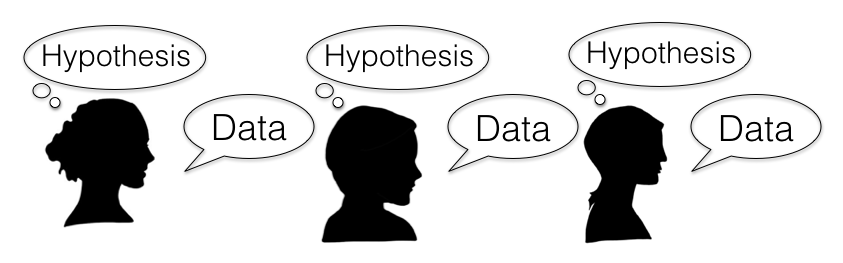
\includegraphics[width=11cm]{iteratedlearningschema.png} 
\caption{{\small Schematic illustration of a typical iterated learning paradigm, which assumes that learner $n$ learns on the basis of the data provided by learner $n-1$. Sillhouette images obtained from http://www.milliande-printables.com/.}}
\label{ilschema}
\end{center}
\end{figure}

One key framework for thinking about and disentangling these two factors is known as {\it iterated learning}, shown schematically in Figure~\ref{ilschema}. Iterated learning is a particular kind of cultural transmission in which behavior arises in one individual (or generation) by learning from the observations of the previous person (or generation) who acquired that behavior in the same way \parencite{kirbyetal14}. As more and more people (or generations) join the chain, we can study the characteristics of the language or the culture that emerges through this process. As a methodology, the technique is old \parencite{bartlett32}, but with increases in the mathematical, computational, and experimental sophistication in its application, it has become considerably more popular in the past decade. 

Although the iterated learning framework is abstract enough to be applicable to the evolution of any kind of cultural knowledge, it has proven especially useful as a way to study the evolution of language. One of the first applications of the paradigm, replicated many times both experimentally and computationally, was to demonstrate that the process of transmission can cause the emergence of compositionality. That is, one can evolve structured languages -- in which different parts of an expression map systematically onto different aspects of meaning -- simply by requiring them to be learned and transmitted from person to person. Several elements are necessary for the emergence of compositionality \parencite{kirbyetal15}. First, there must be a bottleneck or pressure for compression: otherwise languages will become holistic, with distinct, unstructured symbols for each possible meaning rather than structured components whose elements each map onto a part of meaning \parencite{kirby00,brightonetal05,fayellison13}. Second, there must be some kind of pressure for expressivity: otherwise languages will tend to become degenerate, with multiple meanings expressed with the same symbols \parencite{kirbyetal08,perforsnavarro14,silveyetal14}. 

Another application of the iterated learning paradigm is to explain the emergence of regularity in language. Human languages contain a great deal of variation, but that variation is not unpredictable: rather, it is conditioned on phonological, sociological, semantic, or pragmatic factors; truly unconstrained variation is rare or non-existent \parencite{givon85,chambersetal03}. Confusingly, individual adult learners appear to show little or no bias for regularization \parencite{hudsonkamnewport05,vouloumanos08}. If people show little tendency to regularize, how and why do languages evolve to be so regular? The iterated learning framework suggests an answer: models and experiments both demonstrate that weak biases for regularity can be amplified by the process of transmission \parencite{realigriffiths09,smithwonnacott10,smithetal16,morganlevy16}. This is because at each stage of transmission, a weak bias creates an asymmetric pressure in the direction of the bias. Even if each step is small, the effect after many generations is for the bias to be greatly exaggerated and for irregularities to be evened out.

In addition to insights such as these, another advantage of iterated learning is that the abstract behavior of iterated learning chains can be characterized mathematically. One powerful and influential set of results uses the connection between iterated learning designs and the theory of Markov chains to show that under certain assumptions, iterated learning chains will converge to a distribution that depends only on the learners' priors and the size of the bottleneck \parencite{griffiths_language_2007,raffertyetal14}. These analyses all presume that the people in the chain are Bayesian, combining the data they receive from the previous generation with their priors according to Bayes' theorem.\footnote{It is worth noting that in this context, the presumption that people are Bayesian need not be synonymous with a claim that people are rational or optimal. Rather, it refers to a much weaker claim: that their behavior can be described using Bayes' rule, as discussed in \textcite{TauberBIRP}.} On the basis of this mathematical result, iterated learning paradigms have been used in order to reveal what inductive biases people bring to different tasks, including function learning \parencite{kalish_iterated_2007}, visual working memory \parencite{lewvul15}, reasoning about everyday events \parencite{lewandowskyetal09}, and category learning \parencite{caninietal14}.

The analyses of \textcite{griffiths_language_2007} are both fascinating and useful, but they raise a natural question: how do the convergence properties of the chain depend on the mathematical assumptions involved? There has been some work exploring this issue. For instance, we know that chains only converge to the shared prior if people at each generation produce their output by sampling from their posterior distributions; if instead they simply select the hypothesis with the highest posterior probability, then it will tend to exaggerate the prior \parencite{kirbyetal07}. Exactly how much it does so depends on how much data people at each generation see: less data result in greater exaggeration of the prior. This explains both why the presence of a bottleneck changes the outcome of an iterated learning chain, and how weak biases can be magnified through iterated learning. Moreover, iterated learning chains don't always converge to something like the prior or an exaggeration thereof. For instance, all of the previous results have made the assumption that the only input to each person is the previous person in the chain, and that each person generates output without reference to the environment around them. However, we don't use language in a vacuum; we use it to talk about things and events in the world. If one changes the mathematical assumptions to reflect this insight, then the convergent state of the iterated learning chain more closely resembles the posterior distribution over hypotheses given the distribution of things or events in the world \parencite{perforsnavarro14}. 

The possibility that iterated learning chains do not always converge to the prior may cast doubt on those studies which use iterated learning to make inferences about the inductive biases people bring to different problems \parencite{kalish_iterated_2007,lewvul15,lewandowskyetal09,caninietal14}. However, many of these studies do not include anything like an external environment: the assumption that all data are generated by people without reference to the world, inapplicable though it may be to some aspects of real language learning, might appropriately apply in those laboratory experiments. It does raise the question, though, of whether any of the other theoretical assumptions are critical to the idea of convergence to the prior.

Here we investigate the implications of the assumption that all individuals share the same priors and likelihoods. One might assume that this kind of homogeneity shouldn't matter: that ``convergence to the prior distribution'' when priors are heterogeneous should simply mean that the outcome of iterated learning reflects the {\it distribution} of prior beliefs.  For instance, if 10\% of people put all of their belief in hypothesis A and 90\% of people put all of their belief in hypothesis B, one might assume that the convergent distribution will consist of 10\% A and 90\% B. Alternatively, one might assume that the chains will average over the priors, resulting in a convergent distribution concentrated on a hypothesis between A and B.

In this paper we demonstrate that neither of these situations necessarily occurs. If people do not share the same priors, iterated learning does not converge to the prior in any meaningful sense (not even the average). In fact, the stationary distribution to which it does converge is disproportionately influenced by the most biased learners. The same thing occurs when priors are homogeneous but likelihoods are heterogeneous. This has important implications for the interpretation of studies that use iterated learning to draw inferences about people's inductive biases: such experiments may be reflecting the biases of only some of the learners, and distorting even those. It also has important implications for understanding cultural and linguistic change more generally. Perhaps many of the cultural products that we use today may have been shaped by a minority of learners to whom the rest of the population adapts. 

Is this really a worry? Do people actually vary substantially in their priors or likelihoods, particularly in domains like language learning? We would argue that it is, and they do. Indeed, although there may be a few situations where people have roughly homogeneous priors and likelihoods, we suggest that it is {\it those} situations that are a minority. Rather, we argue that most situations involving humans involve substantial individual differences, and that they are reflected mathematically in heterogeneity of priors and likelihoods. 

To see this, consider what it means to specify a prior or likelihood. Mathematically, the prior $p(h)$ corresponds to the weighting an individual puts on the hypotheses in their space before having seen data relevant to the learning situation, while the likelihood $p(d|h)$ does incorporate those data. Thus, the prior captures anything that results in a different weighting of hypotheses at the beginning of a learning situation. Individual differences in memory, attention, executive function, motivation, intelligence, or previous experience thus all have the potential to translate to individual differences in priors because they all have the effect of making different hypotheses more easily accessible, manipulable, conceptualiseable, or useable to some people and not others. The likelihood captures not just the effective data available to the learner (which can be influenced by individual factors such as perception or attention), but also any assumptions made by learners about the data generation process (which can be influenced by factors such as confidence or sampling assumptions). 

Individual differences in these factors are ubiquitous. The literature robustly documents substantial variation in intelligence \parencite{dearyetal00}, working memory \parencite{barrettetal04,unsworthengle07}, executive functioning \parencite{miyakefriedman12}, information processing style \parencite{humphreysrevelle84,epsteinetal96}, learning \parencite{ackerman87, greenwaldetal98}, and decision making \parencite{stanovichwest98,debruinetal07}, among many other things. All of these sources of variation have the potential to translate to effectively different hypothesis weights. 

Within the domain of language, individual differences are also more the norm than the exception. For instance, a recent review paper references hundreds of articles documenting how a wide range of individual differences contribute to differences in language acquisition \parencite{kiddetal17}. These include differences in phonological perception, visual word recognition, syntactic knowledge, prior linguistic experience, working memory, long-term memory, executive attention, efficiency of lexical access, richness of linguistic input, and statistical learning. Most of these things would be expected to manifest as differences in the priors, because they reflect properties of the individual's mind rather than anything to do with the data or assumptions about the data generation process. Moreover, even the most staunchly nativist proponent of Universal Grammar would strongly endorse at least one source of prior heterogeneity: the difference between child and adult learners. 

Overall, individual differences are more the rule than the exception across nearly all domains of cognition, and in many if not most situations these differences may be realised or translated as differences in prior beliefs. Precisely characterising what those differences are and how they translate to priors is far beyond the scope of this paper -- indeed, it is the work of decades. Our focus here is more narrow: when there is variability in priors between people, how does this affect the shape of the distribution that emerges via iterated learning? Given the mathematical generality of the underlying framework, our work is relevant to any situation in which heterogeneous populations of learners transmit data to each other, encompassing (at least in principle) circumstances as divergent as linguistic evolution, the transmission of mathematical knowledge across generations, or what happens in a chain of gossip among friends.

We begin with four simulation studies that highlight how iterated learning chains behave when there are learners with qualitatively different biases, across a variety of situations and within a variety of formalizations. Although details vary, one commonality we observe is that learners with stronger biases have a disproportionate effect on the convergent distribution; to what extent that qualitatively alters the results depends on factors including the nature of the bottleneck and the overall composition of the rest of the populations. We follow the simulations with an illustrative empirical investigation which demonstrates that these effects are substantial enough to make iterated learning untenable as a methodological tool when large individual differences exist.

%In the final section of the paper we consider the broader implications of the work, especially in the context of cultural evolution and language evolution, in which substantive individual differences might be expected to occur, particularly between adults and children or people with different cultural or linguistic backgrounds. 

\section{How do heterogeneous iterated learning chains behave?}

This section outlines four simulations, each of which illustrates a different issue. Our first example investigates regularization of a simple rule, and  illustrates that learners with stronger biases have a larger influence on language change. The second example examines a jury decision making scenario and illustrates how miscalibrated Bayesian learners can exhibit ``groupthink'' behavior. Our third example is a categorization problem that relies on more complex psychological models, illustrating how iterated learning can distort learners' priors when individual differences are present. The final case study presents a systematic exploration of several different factors that might affect the behavior of a heterogeneous iterated learning chain.

\subsection{Case study 1: Who is responsible for regularization?}

Do all learners have equal influence on the process of linguistic and cultural evolution? We consider this question in the context of the emergence of regularities over time. Although in the abstract this situation occurs in a variety of domains -- categories with or without exceptions, constructions with or without irregularities, decision strategies with or without variants -- it arises especially often with regards to linguistic evolution: when, how, and why do regular grammatical or morphological constructions emerge? 

One possible source of heterogeneity is that some learners might have {\sc strong} opinions about a particular rule or construction, whereas others might have {\sc weak} opinions. Exactly who has which opinion might vary with the particular linguistic context and construction involved: for instance, children may have a bias for regularization that adults do not share \parencite{hudsonkamnewport05}, but adult second-language learners may have biases based on transfer from their first language while children do not \parencite{ellis15}. We are fairly agnostic at this point about what such biases might be; all that matters for the present purposes is that it is plausible that there are individual differences in the strength and nature of at least some learning biases. Our question is what effect this might have on the nature of the evolved language or cultural product.

To study this, consider the following iterated learning experiment. Participants are presented with utterances in an artificial language that may incorporate a grammatical feature (e.g., pluralization rule, case marking etc). After training, participants are asked to produce new utterances in this language, and then these utterances are presented as the input to the next learner in the chain. This procedure is relatively typical for linguistic iterated learning experiments, and it corresponds to a simple Bayesian model \parencite{realigriffiths09,smithwonnacott10,ferdinandetal14}.

The model for the task can be constructed as follows. If $\theta$ denotes the probability that the grammatical rule in question should be followed for a novel utterance in the language, then the learner needs to estimate this unknown probability. A Bayesian analysis uses a prior distribution $P(\theta)$ to describe the inductive biases that the participants bring to the experiment, and a standard choice in this scenario is to assume that the prior can be described using a Beta$(a,b)$ distribution in which 
$$
P(\theta) \propto \theta^{a-1} (1-\theta)^{b-1}
$$

The learners with {\sc strong} and {\sc weak} biases can be captured by different priors. In our simulations we formalize learners with a {\sc strong} bias using a Beta(1,10) prior and learners with a {\sc weak} bias with a Beta(2,1) prior. In this scenario, the biases of the two learner types point in different directions, though this need not be true in general.  Regardless of the biases the learner brings to the experiment, it is assumed that belief updating follows Bayes' rule. After completing a training session in which $x$ of the $n$ sentences presented to them follow the rule, the posterior distribution $P(\theta \given x)$ is given by
$$
P(\theta \given x) \propto P(x \given \theta) P(\theta)
$$
where $P(x \given \theta) \propto \theta^x (1-\theta)^{n-x}$ describes the probability of observing $x$ out of $n$ cases satisfying the grammatical rule given that the true probability is $\theta$. Under these assumptions, the posterior over $\theta$ is a Beta$(a+x,b+n-x)$ distribution. When asked to generate a novel sentence for the next learner, a Bayesian learner might choose to sample a value of $\theta$ from their posterior, and their sentences would satisfy the grammatical rule with probability $\theta$. More formally, the number of generated sentences $y$ that satisfy the rule is sampled from the posterior predictive distribution $P(y|x)$:
$$
P(y|x) = \int_0^1 P(y|\theta) P(\theta|x) d\theta
$$
This model is a standard tool when investigating regularization in iterated learning chains \parencite{realigriffiths09,ferdinandetal13}. The posterior predictive distribution supplies the {\it transition probabilities} for an iterated learning chain: if the $i^{th}$ participant is presented with $x$ out of $n$ utterances that follow the grammatical rule, then $P(y|x)$ describes the probability that they will produce $y$ out of $n$ rule-satisfying utterances; these are the utterances that will be presented to participant $i+1$. 

It is natural to expect that the inductive biases of learners will influence the responses that they produce in an artificial language learning experiment. This is illustrated in Figure~\ref{indbias}, which plots the distribution over rule-consistent responses $y$ that we would expect to observe, as a function of two things: the number of rule-consistent training items $x$ plus the nature of the learner ({\sc weak} or {\sc strong}). The {\sc weak} learners have a weak bias to impose the grammatical rule, as illustrated by the fact the response distributions are all shifted slightly to the right hand side of the plots: on average, these learners produce rule-consistent responses slightly more often than they received in the input (i.e., $y>x$). In contrast, the {\sc strong} learners, who have a strong bias against the rule, find the rule hard to acquire. As a consequence they tend to produce far fewer rule-consistent responses in their output than they receive as input (i.e., $y<x$).\footnote{One could perform the same simulation but with {\sc weak} learners who have a bias against the rule and {\sc strong} learners who have a bias to learn it. In that case, the interpretation of the bias would be different but everything else would be identical.}

\begin{figure}[t]
\begin{center}
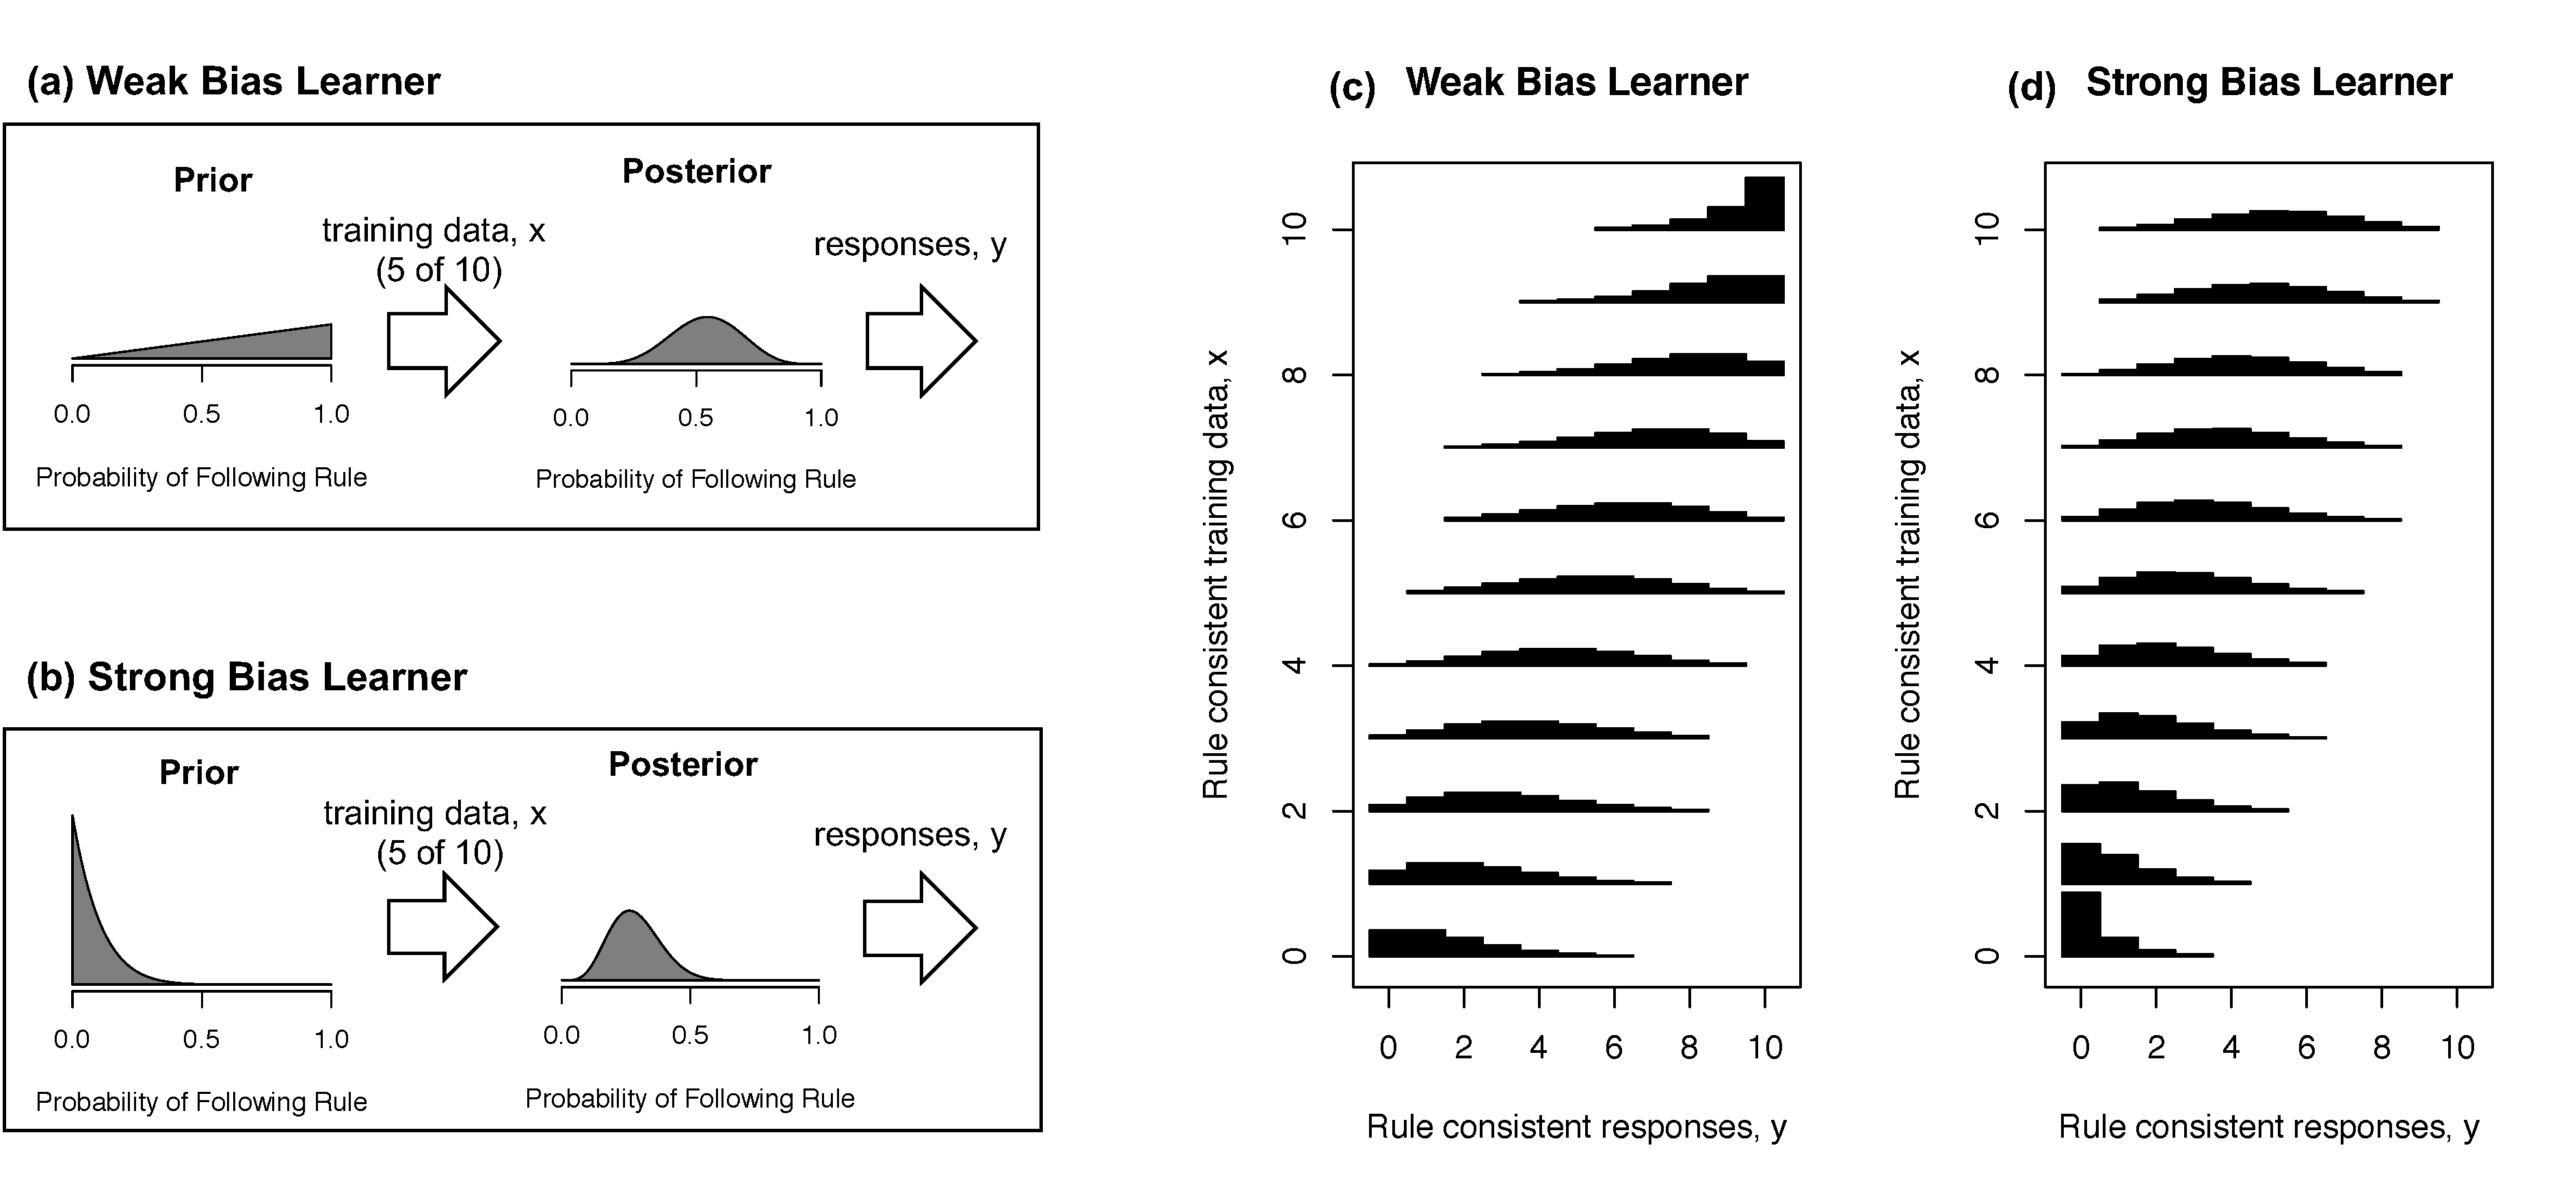
\includegraphics[width=15cm]{bbTrans.pdf} 
\caption{{\small Illustration of the language learning scenario. Each learner is given 10 sentences as input and asked to produce 10 novel sentences as output. Each sentence can be characterized as rule-consistent or rule-inconsistent, with regards to some particular grammatical rule. Panel (a) shows how a learner with {\sc weak} prior bias updates their prior to a posterior distribution when the training data consists of 5 of 10 rule-consistent sentences, and panel (b) shows the corresponding plots for learners with a {\sc strong} prior bias in the opposite direction. The resulting transition matrices for the two learner types are plotted in panels (c) and (d). These panels plot a set of 11 histograms showing the distribution of the number of rule-consistent responses, as a function of the number of rule-consistent input sentences. These plots illustrate the consequences of different inductive biases. Although both learner types tend to mirror the input they receive, the transition matrix for the {\sc strong} bias learner shows a much stronger influence of the prior.}}
\label{indbias}
\end{center}
\end{figure}


\begin{figure}[p]
\begin{center}
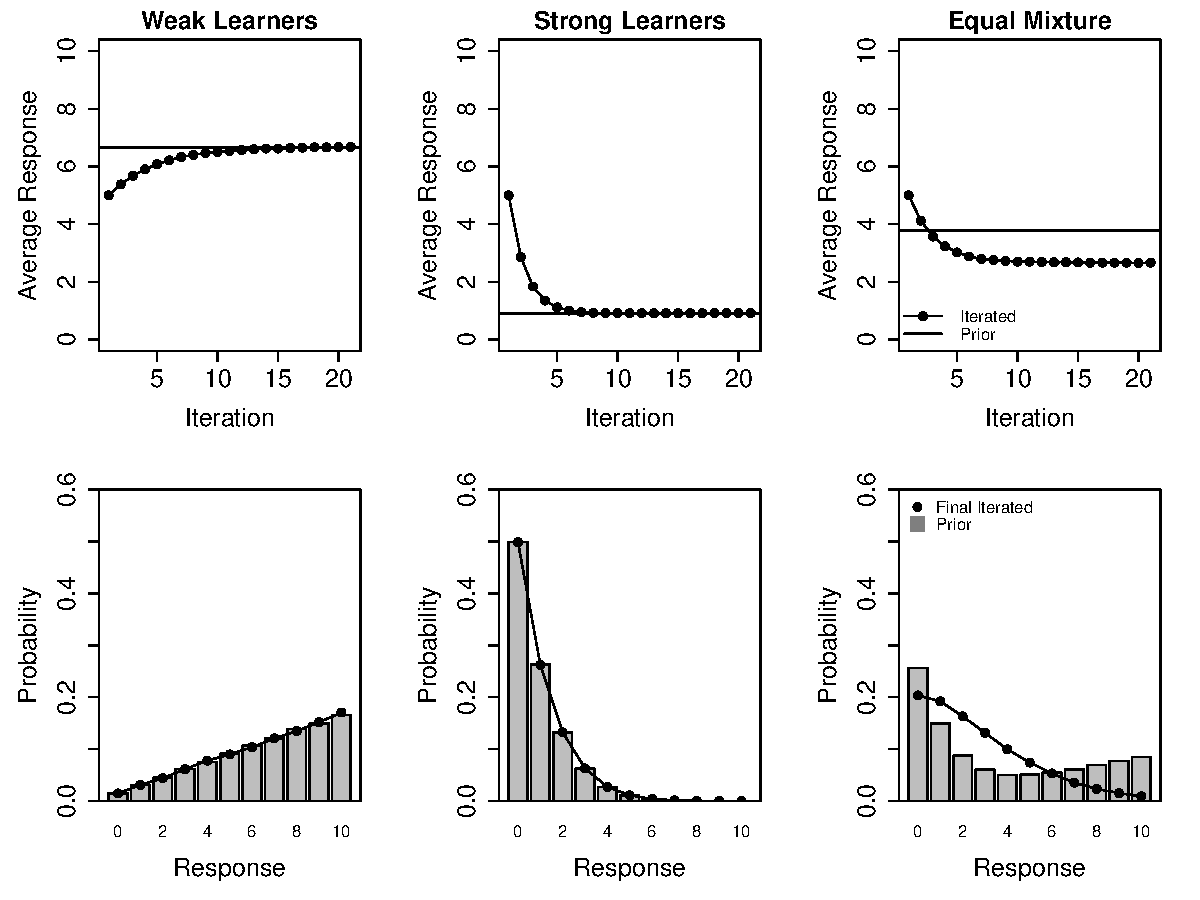
\includegraphics[width=15cm]{coinsfail1.pdf} 
\caption{{\small Iterated learning works when the learners are homogeneous, but fails when they are heterogeneous. The plots on the left show results from an iterated learning chain consisting solely of {\sc weak} learners, and the plots in the middle show the results from an iterated learning chain consisting solely of {\sc strong} learners. The plots on the right depict a mixed chain in which half the learners have a {\sc weak} bias about the general class of grammatical rules to be learned, and half of the learners have a {\sc strong} one. All chains are initialized with 5 of 10 sentences obeying the specific rule in question. The plots in the top row show how the average number (across simulations) of rule-consistent responses produced by the learner changes across generations. The plots in the bottom row show the distribution of responses produced in the 20th generation (solid lines) and the population average prior of the learners (gray bars). The iterated learning chain reveals the true inductive biases (prior) only in the homogeneous chains (left and middle) but produces substantial distortions when the chain is constructed from learners with different biases (right panel).}}
\label{coinsfail1}
\end{center}
\end{figure}

How effectively can iterated learning methods reveal these inductive biases? To answer this question we simulate the results of three different kinds of iterated learning experiments. In all cases, the first person is taught 10 sentences in an artificial language, 5 of which are consistent with a grammatical rule and 5 of which are not; they then generate 10 sentences that are then used as input for the next learner; and so on for a sequence of 20 language learners. In the first experiment all learners are {\sc weak} with the kind of grammatical rule being taught, and in the second experiment all learners are {\sc strong}. In the third experiment, half of the learners are {\sc weak} and half are {\sc strong}. In each case results are aggregated across 100,000 simulated iterated learning chains.

The results are shown in Figure~\ref{coinsfail1}. When all learners share the same inductive biases, an iterated learning experiment transparently reveals those biases. This is illustrated in the left and middle panels of Figure~\ref{coinsfail1}. In the top left panel we see that the {\sc weak} learners tend to regularize: the proportion of rule-consistent responses rises from the initial value of 50\% towards the 67\% probability that the learners expect. Similarly, the iterated learning chain consisting purely of {\sc strong} learners moves in the opposite direction, quickly converging to only 9\% of responses being consistent with the rule, again reflecting the prior bias that these learners possess. The bottom left and bottom middle panels illustrate that, after 20 iterations, the distribution of responses accurately reflects the priors. 

So far this is precisely the pattern of results described by \textcite{griffiths_language_2007}: iterated learning reveals the prior. However, when we consider the iterated learning experiment conducted with a mixed population (right panels of Figure~\ref{coinsfail1}), we observe a strikingly different result. In this situation -- where half of the learners are {\sc weak} and half are {\sc strong} -- the average bias in the population is to expect 38\% of sentences to be rule-consistent. Yet, as the top right panel shows, the iterated learning chain converges to a smaller number, with only 27\% of responses following the rule. More importantly, as the bottom right panel reveals, the distribution of responses bears very little resemblance to the underlying population biases. One might have hoped that, when learners bring different priors to an iterated learning experiment, the chain would converge to a weighted average of their priors. In this case, this weighted average would be a 50-50 mixture of the priors of {\sc weak} learners and {\sc strong} learners, which is shown by the dots-and-lines. As the figure illustrates, the iterated learning chain (histogram) does not converge to anything even remotely similar to this mixture distribution.

\begin{figure}[t]
\begin{center}
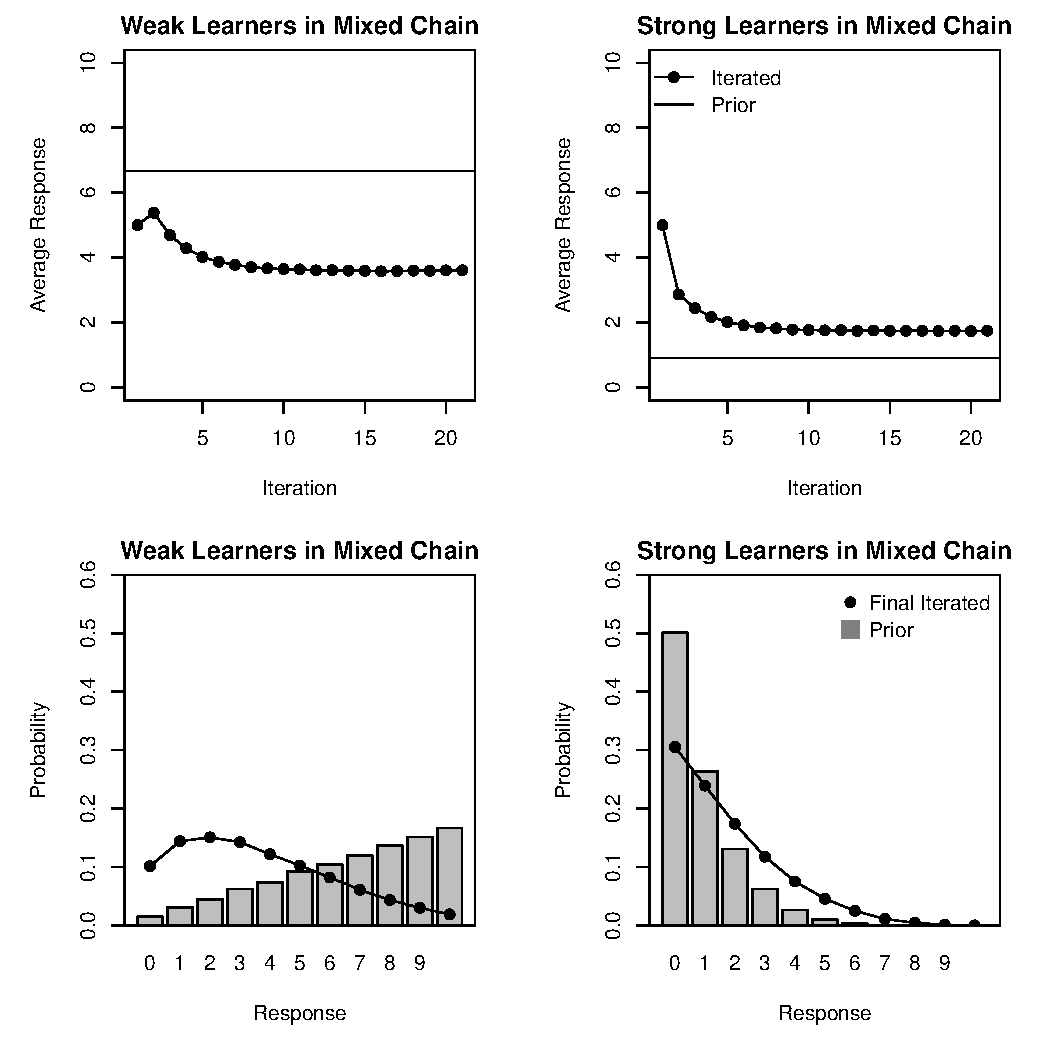
\includegraphics[width=11cm]{coinsfail2.pdf} 
\caption{\small{Responses in the mixed chain broken down by learner type. The {\sc weak} learners produce responses (top left panel, dotted line) that are quite different from those that they would have produced in a homogeneous chain (top left panel, solid line). Nor does the distribution of their responses (bottom left panel, dotted line)  reflect the distribution of their priors (bottom left panel, bars). By contrast, the {\sc strong} learners produce responses that are more similar to those they would have produced in a homogeneous chain and to their prior distribution. The {\sc weak} learners are more profoundly distorted by being in a chain with {\sc strong} learners, rather than vice-versa.}}
\label{coinsfail2}
\end{center}
\end{figure}

Why does the iterated learning procedure fail to reveal ``the prior'' when the population is heterogeneous? An answer to this question can be found by separating the responses by learner type, shown in Figure~\ref{coinsfail2}. The left hand side of the plot shows the response distributions produced by {\sc weak} learners in the mixed chain; they do not look at all similar to the responses that they would have produced in a homogeneous chain. Instead of converging to their own prior bias, which would give rise to 67\% rule consistent responses, their responses are very strongly influenced by the the biases of the {\sc strong} learners, and as a result their responses are rule-consistent 36\% of the time. However, this effect is not symmetric: the influence of the {\sc weak} learners increases the number of rule-consistent responses of the {\sc strong} learners by a much smaller amount, from 9\% to 17.5\%. The distributional effects shown in the lower panels are even more pronounced: by the final iteration of the experiment, a {\sc strong} learner can be expected to sample responses from a distribution that is not markedly different from their prior, but the responses produced by a {\sc weak} learner are drawn from a distribution that is qualitatively different from both their prior and the group's average prior. 

As this simple example illustrates, when individual differences exist an iterated learning procedure is not guaranteed to reveal the inductive biases of the learner in any meaningful sense of the term. The reason this occurs is that the {\sc strong} learners apply a very strong inductive bias: the Beta(1,10) prior that they bring to the learning problem ensures that these learners require a lot of evidence before they are willing (or able) to apply the grammatical rule in question, and as a consequence data generated by a {\sc weak} learner will have minimal ability to sway such a person. The reverse does not hold: the {\sc weak} learners in this scenario adopted a Beta(2,1) prior that ensures they have a prior bias to expect a grammatical rule, but this bias is weak and these learners are very responsive to external input. As a result, a {\sc weak} participant makes a much larger adjustment from the prior than does an {\sc strong} one, with the consequence that the overall behavior of the mixed chain is much more heavily driven by the group with the strongest bias.

This result is robust, perhaps also underwhelming: after all, these average responses are different from the averaged priors but not strikingly so, and the overall proportion of rule-consistent responses has not changed a great deal. However, consider what happens when the vast majority of the population consists of completely unbiased learners with a Beta(1,1) prior but 5\% consists of learners with a Beta(100,1) prior that strongly favors adopting the rule. In that situation, shown in the top row of Figure~\ref{coinsfail4}, the population-level response appears far more extreme than the vast majority of learners, following the rule almost 80\% of the time (left panel). The middle and right panels show that this is because, as previously, the less extreme Beta(1,1) learners systematically adopt the rule far more than their prior would suggest they do. The more extreme Beta(100,1) learners under-adopt relative to their prior, but not as much, so the population average behaviour is distorted.\footnote{Interestingly, the output of the iterated learning chain also does not converge to a weighted population average in which weights correspond to strength of belief. We tested this by weighting each learner proportional to the number of prior pseudo-observations; thus, a weighted mixture of a Beta(98,2) and a Beta(1,49) would assign twice as much weight to the former than the letter. The chain slightly undershot this value. It would be possible to calculate weights in other ways (e.g., entropy of priors, etc) but for space reasons we omit a fuller exploration of these possibilities. In any case it is clear that the nature of the convergent distribution is not obviously predictable.}

Some readers may have noticed one apparent discrepancy between our results and other work showing that the long-run behaviour of iterated learning chains such as these is toward complete regularization and full adoption of a rule or pattern \parencite{realigriffiths09,smithwonnacott10}. The reason we do not observe that here is that so far we have assumed that learners sample their hypotheses from the posterior distribution rather than picking the one with the highest posterior probability. This latter process, known as MAP learning, has been shown to exaggerate the prior \parencite{kirbyetal07}. 

\begin{figure}[p]
\begin{center}
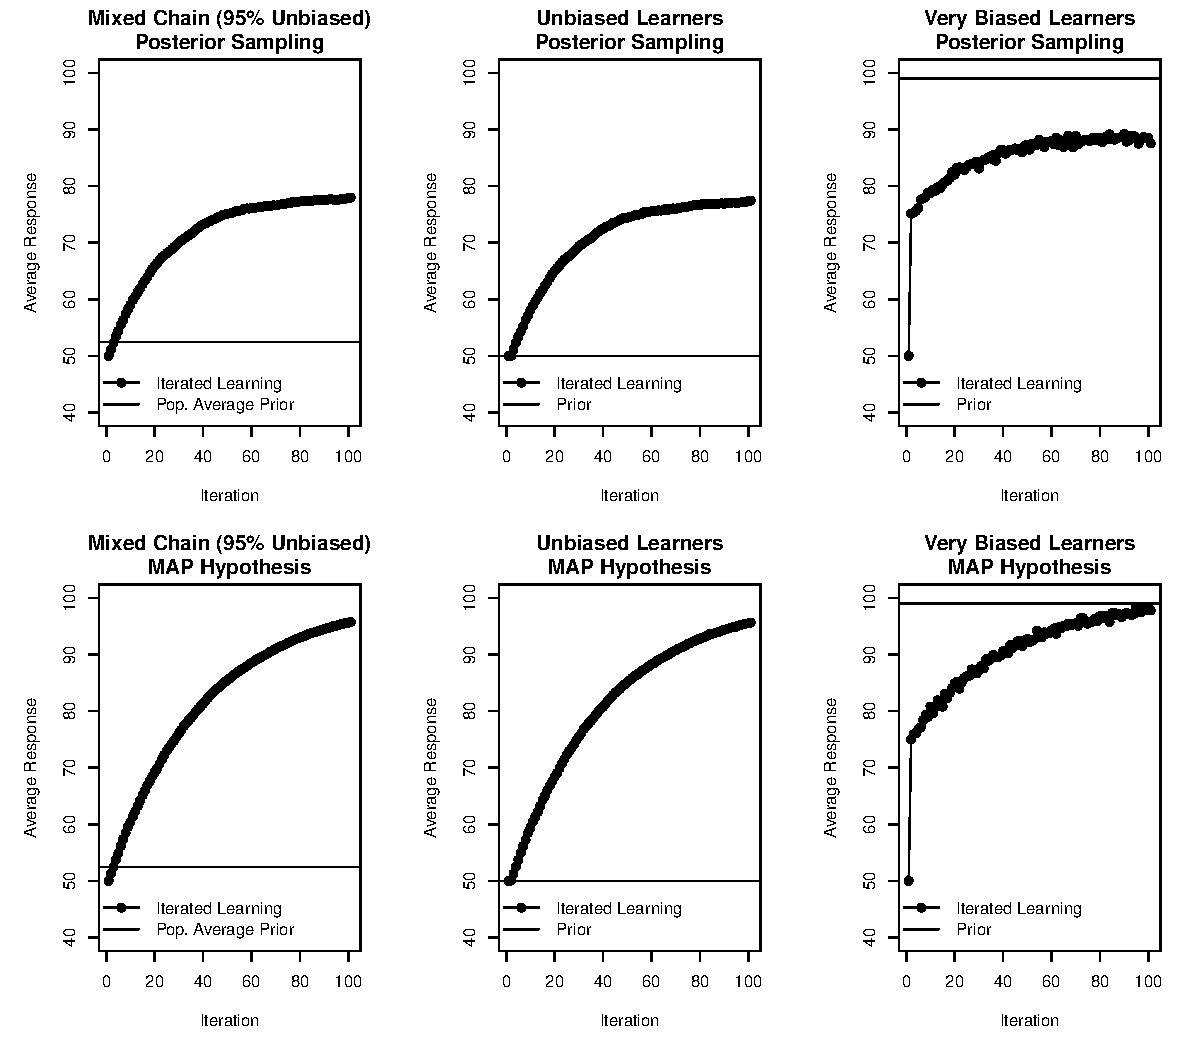
\includegraphics[width=14cm]{coinsfail4.pdf} 
\caption{\small{Linguistic rule adoption when the population of learners is highly uneven. In this scenario, 95\% of learners are unbiased and 5\% have a very strong prior to adopt the rule. The top row assumes that learners sample their hypotheses from the posterior distribution, while the bottom row assumes they pick the one with the highest posterior probability (MAP learning). The left column shows the behaviour of this mixed chain: even though 95\% of the learners are unbiased, the chain ends up producing the rule about 80\% of the time when learners sample from the posterior (top left), and almost complete regularization when learners apply MAP learning (bottom left). This occurs because the responses of the unbiased learners (middle column) are significantly distorted from their priors, as a result of occasionally receiving input from the biased learners (right panel), who are not distorted nearly as much.}}
\label{coinsfail4}
\end{center}
\end{figure}

What happens to an iterated learning chain with a mixed population of MAP learners with a heterogeneous set of priors? The bottom row of Figure~\ref{coinsfail4} explores this question with a population identical to the top row but making the assumption that the learners produce output by selecting the hypotheses that maximize posterior probability rather than sampling from the posterior distribution. It is clear that the amount of distortion caused by the tiny 5\% minority of extremists has been exaggerated even further: even though only a few have any bias towards the rule at all, it is enough to produce almost complete adoption of the rule by all learners by the 100th iteration of the chain. This result is especially interesting in light of previous work suggesting that iterated learning can result in full regularization even if everyone in the population has only weak priors for regularization  \parencite{smithwonnacott10}. Our result suggests that regularization can emerge even if the vast majority of individuals in the population are not biased {\it at all} to regularize. More broadly, the theoretically interesting implication of this entire case study is that as long as there are different people in a population with different biases, it is those with the stronger ones that have a disproportionate effect on the resulting language. Depending on the rule or construction involved, such people might be children, adult second language learners, or individuals from a culturally dominant subgroup. 

%In our simulations the {\sc weak} learners had a slight bias to follow a given rule while the {\sc strong} learners strongly preferred not to, but the critical point is about the strength rather than the nature of the bias: the same qualitatively conclusions would apply in the other direction if the {\sc strong} learners had a preference to drop the rule. 


%correspond to adult participants from a language community that possesses a similar grammatical rule to an artificial language, and the {\sc strong} learners are adult participants speak a language without that feature (as might occur during the formation of a creole), but the implications for language evolution are much broader. Another way that the same pattern can arise is when some learners are adult speakers that are {\sc weak} with the current structure of a language, and others are children that are {\sc strong} with it. To the extent that a lack of knowledge, memory constraints, and other limitations that younger children make them similar to the {\sc strong} group in our scenario, we should expect them to have a disproportionate influence on cultural and linguistic evolution.

How much do these results stem from the particular details of our formalization? To address this question, the next case study considers another kind of heterogeneous population in which people differ in the degree to which they depend on their own reasoning rather than relying on others. This technically corresponds to heterogeneity in likelihoods rather than priors, but as we shall see, the effects are similar: the resulting distribution is disproportionately shaped by some agents over others. 

\subsection{Case study 2: Phrenology, forensics and the overconfident crowd}

Communities of learners often arrive at beliefs that seem entirely unfounded in evidence Examples include the widespread belief in phrenology in the 19th century \parencite{faigman2007anecdotal}, disproportionate trust in unreliable forensic methods \parencite{pcast2016}, beliefs in conspiracy theories \parencite{goertzel1994belief}, and ``groupthink'' that plagues decision making processes \parencite{janis1982groupthink}. How do these false beliefs arise? Do they necessarily reflect an overly-credulous form of reasoning that all humans are equally susceptible to, or can an entire community of mostly well-calibrated learners be misled by a small number of highly biased learners? 

To illustrate how this might work, consider the following scenario in which a jury of 12 people begin their deliberations with a straw poll. A notepad is passed around the room, with each person writing down whether they would decide in favour of the plaintiff or the defendant before removing their sheet of paper and passing the pad to the next juror. Unfortunately, it turns out that paper on the notepad is rather thin, and each juror can clearly read the indentations left by the previous person. Therefore, the straw poll forms an iterated learning chain in which each juror receives input from the previous one. 

Clearly, the flawed notepad creates a situation that violates the independence of the juror votes in the straw poll, but does it distort the overall results? To answer this, we consider the behavior of a simple Bayesian juror. The juror considers two hypotheses, namely that the evidence favors the plaintiff ($e=1$) and that it favors the defendant ($e=0)$. On the basis of their personal evaluation of the evidence at trial, the juror believes that the outcome should favor the plaintiff with probability $\theta$. This belief sets the juror's prior belief, $P(e=1)=\theta$, a belief that is updated when the notepad is passed to them and the vote $v$ of the preceding juror is inadvertently revealed. The juror unconsciously assigns a reliability $r$ value to the previous person, such that $P(v=1|e=1) = P(v=0|e=0) = r$, and updates their beliefs accordingly. If the preceding juror voted for the plaintiff, the current juror's posterior degree of belief that the verdict should favor the plaintiff becomes
\begin{equation}
P(e=1 \given v=1) = \frac{r\theta}{r\theta+ (1-r)(1-\theta)}
\label{sheepgoat1}
\end{equation}
whereas if the earlier vote favored the defendant, this posterior probability becomes
\begin{equation}
P(e=1 \given v=0) = \frac{(1-r)\theta}{(1-r)\theta + r(1-\theta)}
\label{sheepgoat2}
\end{equation}
For simplicity, we assume that the juror generates their own vote probabilistically, by sampling from the posterior distribution: if the juror's posterior indicates that there is a 95\% probability that the evidence favors the plaintiff, then they vote in favor of the plaintiff with probability 0.95. As these equations illustrate, when $r=0.5$ the current juror completely ignores the vote provided by the previous one and the posterior probability is identical to the prior. This arises naturally when the current juror is confident that their existing beliefs incorporate all relevant information about the case, and as such the opinions of other jurors can have no influence upon their own beliefs. We refer to such a juror as a {\sc goat} -- someone who forms their own view and is not led to conclusions by the opinions of others. In contrast, suppose the juror is underconfident about their beliefs, perhaps suspecting that other jurors have access to different information. Such a juror will set $r>0.5$, because they attribute evidentiary value to the opinions of others, and we refer to this kind of a juror as a {\sc sheep} because they are more likely to adjust their vote to agree with the votes of others. Note that {\sc sheep} in this case are mis-calibrated: since the juror next to them saw no different evidence than they did, by taking their opinion into account they are treating non-independent data (the evidence in the trial and the neighbouring juror’s belief) as independent and overweighting that evidence. What happens in this case? 

We consider three scenarios for how this straw poll may play out. In the first scenario all jurors are {\sc goats} who set $r=0.5$ and have a modest opinion in favor of the defendant ($\theta = 0.4)$. In the second scenario all jurors are {\sc sheep} who set $r=0.9$ and have a modest opinion favoring the plaintiff ($\theta = 0.6$). Finally we consider a situation where half of the jurors are {\sc sheep} and the other half are {\sc goats}. To illustrate what happens in these situations we simulated each scenario 100,000 times. The results are plotted in Figure~\ref{juror}. Not surprisingly, because the {\sc goat} jurors ignore the input and generate responses directly from their own prior beliefs, the ``chain'' starts at their prior (on average, 40\% of jurors vote for the plaintiff) and the total number of votes in favor of the plaintiff follows a binomial distribution.


\begin{figure}[t]
\begin{center}
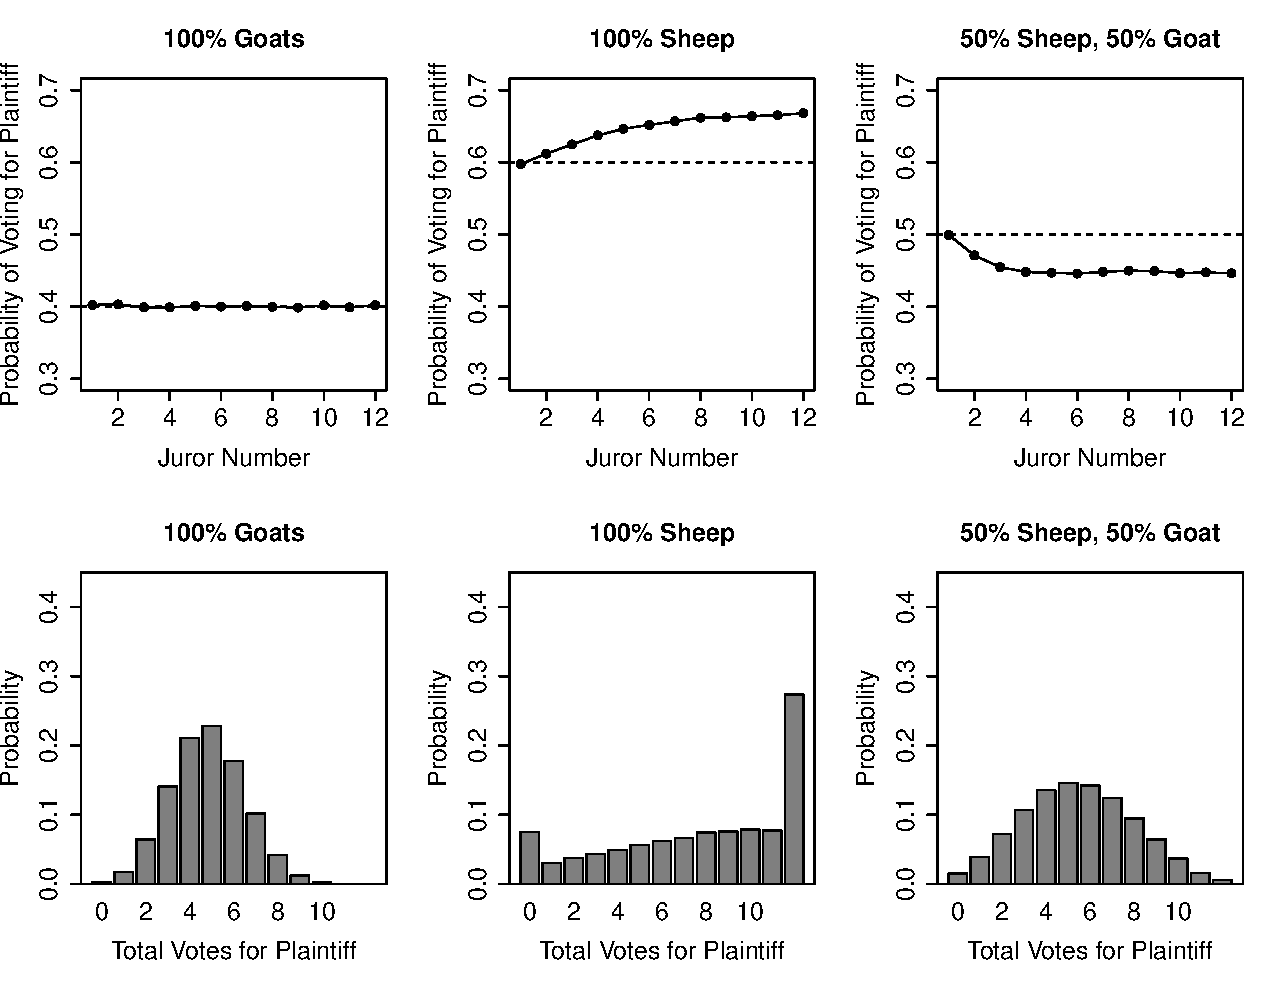
\includegraphics[width=14cm]{juror1.pdf} %\includegraphics[width=7cm]{brn2.pdf}
\caption{{\small The results of the hypothetical jury straw poll. The top row plots the probability that each juror votes for the plaintiff, as a function of their position in the chain (the dashed line plots the population average prior in each case), and the bottom row plots the distribution (across simulations) of the total number of votes for the plaintiff. Plots on the left show the results if all jurors are {\sc goats}, the middle column shows the results if all jurors are {\sc sheep}, and the results on the right show the outcome if half of the jurors are {\sc goats} and the other half are {\sc sheep}.}}
\label{juror}
\end{center}
\end{figure}


What should we expect to see if all jurors are {\sc sheep}? One reading of the literature suggests that, since iterated learning chains of Bayesian learners converge to the prior, and since the first {\sc sheep} samples from their own prior, we should see a result not dissimilar to the one we see for {\sc goats}. That is -- while we might expect to see non-independence among successive jurors -- we should find that on average a {\sc sheep} juror should vote for the plaintiff 60\% of the time, in accordance with their priors. However, as the middle column to Figure~\ref{juror} illustrates, this is emphatically not what happens. The first juror does indeed vote in accordance with their priors, but by the time the 12th juror is polled, the probability of voting for the plaintiff has risen to about 67\%. Moreover, it is very simple to prove that this is not a simulation error. A pure iterated learning chain of {\sc sheep} does not converge to the prior in any meaningful sense. The long-run probability of a {\sc sheep} voting for the plaintiff is in fact 2/3. Let $p = P(v_i=1 | v_{i-1}=0)$ denote the probability that the $i^{th}$ juror in the chain votes for the plaintiff given that the previous juror voted for the defendant, and similarly let $d = P(v_i = 0 | v_{i-1}=1)$ denote the probability that the $i^{th}$ juror switches the other direction. The transition matrix for the strawpoll is thus 
$$
\bm{T} 
= \left[ \begin{array}{cc} 1-p & p \\ d & 1-d \end{array}\right]
$$
A Markov with this transition matrix converges to a stationary distribution $\bm{\pi}$ in which the (marginal) probability of voting for the defendant and plaintiff is proportional to $d$ and $p$ respectively. To verify this, note that 
\begin{eqnarray*}
\bm{\pi} \bm{T}  &\propto& [d, p] \left[ \begin{array}{cc} 1-p & p \\ d & 1-d \end{array}\right] \\
&=& [d(1-p) + pd, dp + p(1-d)] \\
&=& [d, p]\\
&\propto& \bm{\pi}
\end{eqnarray*}
It is straightforward to use Equations~\ref{sheepgoat1} and \ref{sheepgoat2} to show that for a {\sc sheep} juror, the probability of switching the vote from the plaintiff to the defendant is $d = (.1 \times .4) / (.1 \times .4 + .9 \times.6) = .069$, and similarly the probability of switching the vote towards the plaintiff is $p = (.1 \times .6) / (.1 \times .6 + .9 \times.4) = .142$. Accordingly, in the long run, a chain of {\sc sheep} converges to a 67\% probability of voting for the plaintiff even though each individual {\sc sheep} only assigns a 60\% prior probability to the plaintiff. 

%0.034
%0.073

To understand why this result occurs -- in seeming violation of the convergence proofs offered by \textcite{griffiths_language_2007} -- note that the distribution of {\sc sheep} votes in the lower middle panel of Figure~\ref{juror} is bimodal. In almost all cases {\sc sheep} vote as a block: the most likely outcome is that all 12 jurors vote for the plaintiff, but should that not occur the second most plausible outcome is all 12 jurors voting for the defendant. Ultimately this occurs because the {\sc sheep} jurors are fundamentally miscalibrated. Because the {\sc sheep} juror assigns evidentiary value to the opinions of other jurors -- even though those other jurors have observed the exact same evidence at trial -- the strength of their posterior belief in the plaintiff's case is exaggerated. In effect they have ``double counted'' the evidence at trial: the evidence at trial is used to form the current juror's prior opinion, but because that same evidence {\it also} influenced the vote of the previous juror, it can also exert an indirect influence on the current juror. As a consequence, an iterated learning chain constructed solely from {\sc sheep} jurors does not converge to the prior.

Next, consider what happens when {\sc sheep} and {\sc goats} are mixed together in equal proportions, as depicted in the right hand column of Figure~\ref{juror}. The {\sc sheep} assign prior probability of 0.6 to the plaintiff, whereas the {\sc goats} assign prior 0.4, so the population average prior is 0.5. Alternatively, if we consider the behavior of the two homogeneous iterated learning chains, the {\sc sheep} on their own would be expected to converge to 0.67 and the {\sc goats} would converge to 0.4, so the average of these two long run probabilities is 0.54. It would not be unreasonable -- if one did not know the details -- to expect that an iterated learning chain comprised of an equal mixture of these two learner types should converge to a situation in which the average probability of voting for the plaintiff should lie somewhere between 50\% and 54\%. Unsurprisingly, of course, it does nothing of the sort. Because the {\sc goats} are insensitive to the opinions of others whereas {\sc sheep} are highly influenced by others, the {\sc goats} dominate the behavior of the mixed chain, and the long run behavior converges to a 43\% probability of voting the plaintiff. This is shown more clearly in Figure~\ref{juror2} which shows exactly this asymmetry: the {\sc sheep} ``learn'' to mimic {\sc goats} but the {\sc goats} make no such accommodation.

\begin{figure}[t]
\begin{center}
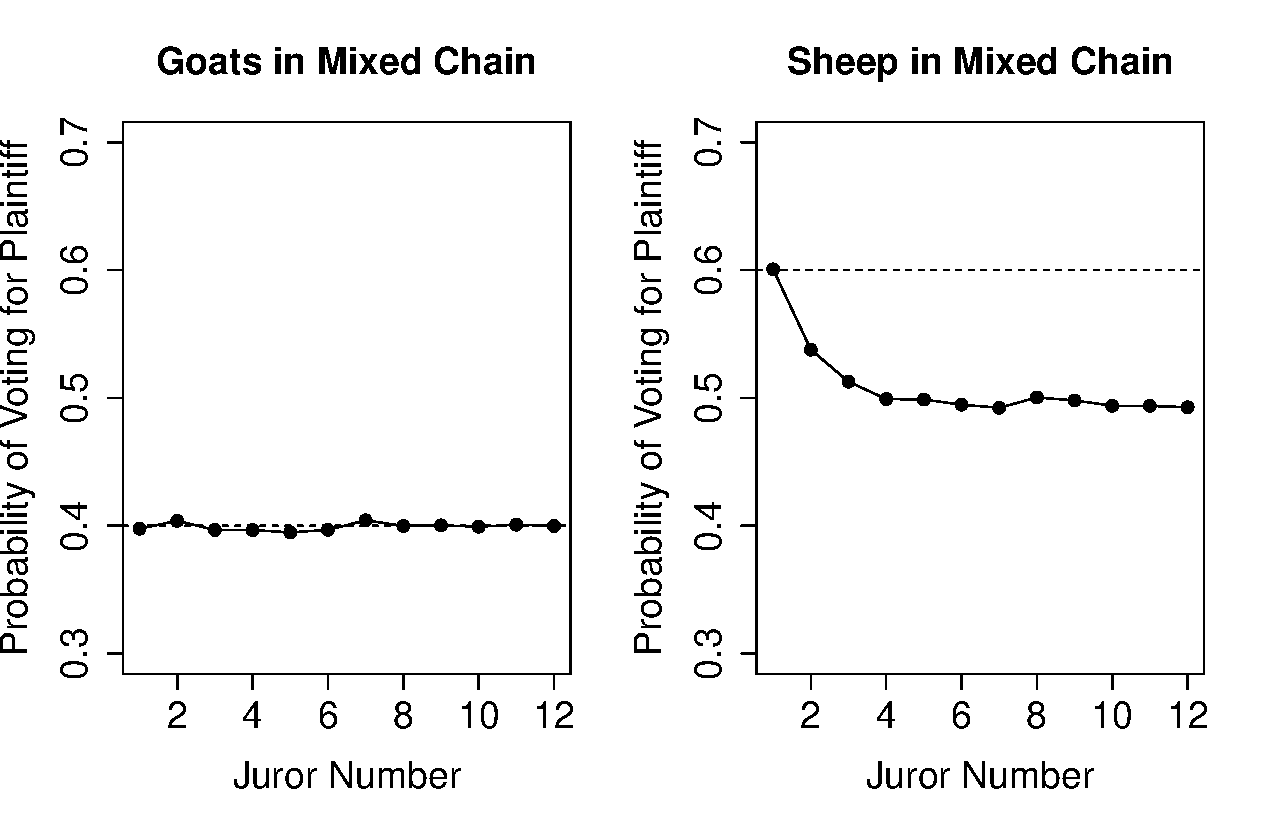
\includegraphics[width=10cm]{juror2.pdf} %\includegraphics[width=7cm]{brn2.pdf}
\caption{{\small The behavior of {\sc sheep} and {\sc goats} when mixed together in the jury scenario. As one might expect, the behavior of {\sc goats} is entirely unchanged by the presence of {\sc sheep}, but the {\sc sheep} shift their votes to more closely match the {\sc goats}.}}
\label{juror2}
\end{center}
\end{figure}

Although this simulation describes a very simple situation, it highlights two important things about how iterated learning scenarios can play out. Firstly, the {\sc sheep}-only scenario illustrates that even in the homogeneous case where all learners are identical to each other, it is possible for an iterated learning chain to converge to something other than the prior. This result mirrors previous work by \textcite{smith2009iterated} showing that convergence can be affected when learner's likelihood function is at odds with the true generative process. Relatedly, it complements work by \textcite{perforsnavarro14} which showed that the convergence of iterated learning chains is affected when there is an additional input to the chain (i.e., the world passes new information to learners). In the {\sc sheep} chain we find that convergence is influenced when learners mistakenly {\it believe} there is additional information being passed into the chain. This mistaken belief drives a kind of groupthink, in which a collection of individually {\it underconfident} learners becomes {\it overconfident} as a group. That is, because each {\sc sheep} has insufficient confidence in their own priors, an iterated learning chain of {\sc sheep} jurors becomes overly confident. In essence, this result provides a mechanism for a very strong belief to emerge in a fashion that is not driven by the external world, and moreover that it is fundamentally caused by the underconfidence of individual learners. 

The second point to take away from this simulation is that the behavior of a heterogeneous chain is not easily predicted by considering the behavior of its constituent homogeneous chains, or the priors of individual learners. The mixed chain of {\sc sheep} and {\sc goats} is much more strongly driven by the {\sc goats}, even though a homogeneous chain of {\sc goats} produces a much less extreme outcome than the a chain of pure {\sc sheep}. People who are more willing (or able) to learn from the input of others will have {\it less} influence on an iterated learning chain than people who do not adjust their beliefs. This asymmetry is shown very clearly in the {\sc sheep-goats} scenario here, but it is the same phenomenon that drives the asymmetry between the {\sc weak} and {\sc strong} learners in the first case study. 

\subsection{Case study 3: Categorization}

The examples considered to this point have focused on Bayesian models and situations in which where there are two qualitatively different groups in the population. Our third case study expands the focus, and considers a situation involving non-Bayesian models and a more general notion of individual differences. The problem we focus on is categorization, and we use a standard exemplar model (Nosofsky, \citeyear{nosofsky_attention_1986}) of classification to highlight how iterated learning plays out in this setting when the population is heterogeneous. 

We consider a learning problem in which stimuli vary along a single stimulus dimension with 8 exemplars spaced evenly across the range (located at $x=1,\ldots,8$). Each of these items can be assigned to one of two categories (A or B). We are interested in exploring the presence of two different kinds of inductive biases, one pertaining to category {\it size} and another pertaining to category {\it coherence}. The ``category size'' bias refers to whether the learner has an {\it a priori} preference to divide the stimuli into two equally sized categories (e.g., a 4-4 split) or prefers to divide them in a more uneven fashion (e.g., a 7-1 split). The ``category coherence'' bias refers to the extent to which the learner prefers to group similar (i.e., nearby) items into the same category. 


\begin{figure}[t]
\begin{center}
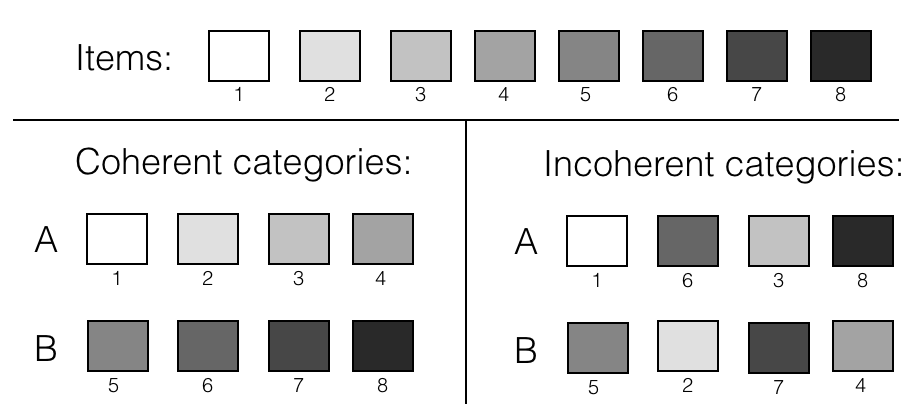
\includegraphics[width=9cm]{categorisation.png} %\includegraphics[width=7cm]{brn2.pdf}
\caption{{\small In case study 3, we consider a categorization case with eight items from two categories that differ from one another along one dimension (top panel). We imagine a situation in which an experimenter might want to use the iterated learning task to infer to what extent people have a bias to assume that categories are coherent (left panel) rather than incoherent (right panel).}} 
\label{categories}
\end{center}
\end{figure}


An iterated learning design can be used to explore these biases in a relatively straightforward way, as illustrated in Figure~\ref{categories}. During category learning, each learner is shown training items that consist of four exemplars and their category labels, selected randomly subject to the constraint that there must be one exemplar of each category in the training set. During the test phase the learner must classify the remaining four exemplars. An iterated learning chain is then constructed in an obvious way, by using a random subset of responses from one learner as the training data for the next, subject to the constraint that the learner must be shown at least one example of each category. To simulate the behavior of the chain, we assume each participant can be modeled using the Generalized Context Model (GCM) of Nosofsky (\citeyear{nosofsky_attention_1986}). According to the GCM, the probability of assigning a test item located at $y$ to category A given training items $\bm{x} = (x_1,\ldots,x_n)$ with labels $\bm{l} = (l_1, \ldots, l_n)$ is proportional to the sum of the similarities between the test item and the known members of category A:
$$
P(y \in A \given \bm{x}, \bm{l}) = \frac{\sum_{i | l_i = A} S(x_i,y)}{\sum_{i | l_i = A} S(x_i,y) + \sum_{i | l_i = B} S(x_i,y)}
$$
Exemplar similarity is an exponentially decaying function of distance in the psychological space:
$$
S(x,y) = \exp( -\lambda |x-y|)
$$
The model has one free parameter: the {\it specificity} parameter $\lambda$, which describes how rapidly similarity decays as a function of distance. When $\lambda$ is large, similarity falls away very quickly with distance, and when $\lambda$ is small similarity diminishes much more slowly. Although the GCM is not usually framed as a Bayesian model (but see Nosofsky, \citeyear{nosofsky_relation_1991}) it nevertheless imposes inductive biases that ensure that some categorization schemes are a priori more ``natural'' than others \parencite{pothos_predicting_2009}. Moreover, these biases are dependent on the value of the specificity parameter $\lambda$, a fact that becomes very apparent when we simulate the behavior of (homogeneous) iterated learning chains using GCM learners. 

To illustrate this, consider the category coherence bias. Let AAAABBBB denote the category structure in which the four items located at $x=1,2,3,4$ belong to category A, and the other items belong to category B (left panel in Figure~\ref{categories}). The category structure AAAABBBB has the maximum possible coherence, while the maximally incoherent category structure is one in which the labels alternate ABABABAB. A simple way of measuring the coherence of a categorization scheme is to count the number of times a pair of adjacent items are assigned to the same category. There are no instances of this occurring for the ABABABAB structure, so it has coherence zero. For AAAABBBB, there are six such instances. Using this measure, it is possible to obtain a very clear picture of how the GCM imposes a coherence bias within an iterated learning design. The left panel of Figure~\ref{catcoherence} shows what happens in an iterated learning chain when all participants have the same $\lambda$. The first learner is shown a random subset of four items and asked to label the other four; those responses were used to generate the input for the next learner. At the beginning of all chains, when the category assignments are random, the average coherence is the same regardless of $\lambda$. When similarity decays slowly ($\lambda=0.1$) the GCM does not impose a strong coherence bias on the input, and the stationary distribution of the chain reflects that: the categories produced by the iterated learning chain are only barely more coherent than random assignment. In contrast, when we set $\lambda=10$, corresponding to a narrow generalization gradient, the GCM always assigns items to the same category as the nearest exemplar. This creates a strong pressure towards maximally coherent category structures, and the iterated learning chain converges to a coherence value of six.

Of course, the assumption that all of the learners have the same prior seems unlikely to apply to humans. With that in mind we ran a second simulated iterated learning study, shown in the right panel of Figure~\ref{catcoherence}. This time we allowed learners to vary in their $\lambda$ values (sampling uniformly at random from the same three $\lambda$ values of 0.1, 1,  and 10). In the figure, the gray dotted line reflects the  average of this heterogeneous population of learners over the course of iterated learning. It is apparent that it is lower than the average of the learners when they are in homogeneous chains (on the left). Overall, however, when we compare the left and right panels to one another the impression is that the differences are modest. All the learners become somewhat more similar to one another, with the categories produced by $\lambda=10$ learners becoming slightly less coherent and the curves for the $\lambda=0.1$ learners becoming slightly more coherent; but the average coherence does not change by much. Based on this figure, one might conclude that the heterogeneity of the population has done very little to distort the categorization schemes produced by the various different learners. Unfortunately, this conclusion would be incorrect, as becomes apparent when we consider a different inductive bias.


\begin{figure}[t]
\begin{center}
\begin{tabular}{c}
\textsf{Category Coherence} \\
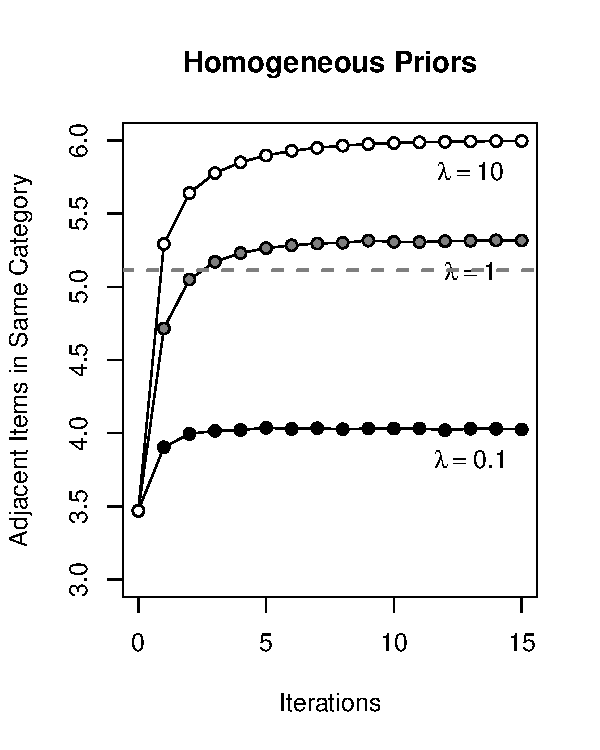
\includegraphics[width=6cm]{catcohpure.pdf} 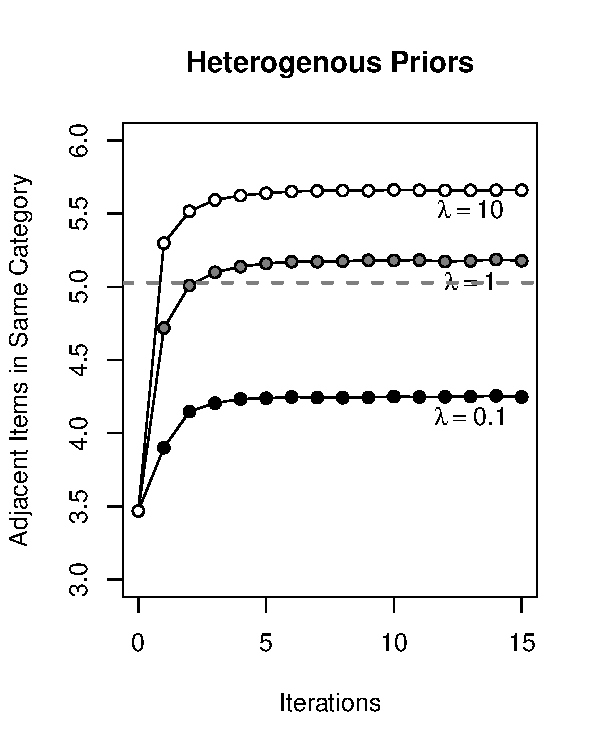
\includegraphics[width=6cm]{catcohmixed.pdf}
\end{tabular}
%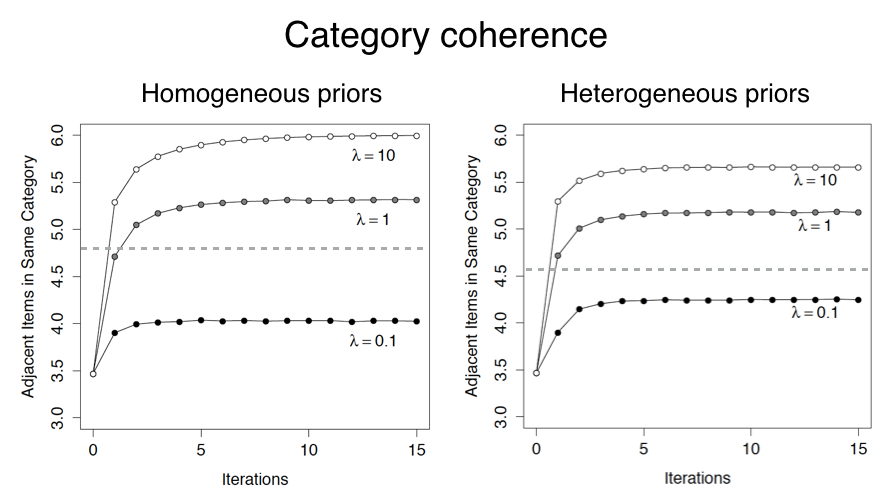
\includegraphics[width=12cm]{catcohall.png}
\caption{\small{Category coherence: Performance of iterated learning chains in a supervised learning categorization task. The $y$ axis shows category coherence as reflected in the number of adjacent items in the same category: higher numbers reflect more coherence. {\bf Left panel}: Category coherence assuming all participants share the same prior ($\lambda$). Here there are three chains each reflecting one of the three $\lambda$ values. As $\lambda$ grows higher, iterated learning produces more coherent categories. The gray dotted line reflects the average of the three chains. {\bf Right panel}: When there are individual differences within participants, the overall average coherence of the iterated learning chain (gray dotted line) is lower than the average coherence of the three participant types taken separately (gray dotted line in left panel). This is because the behavior of learners with larger $\lambda$ is pulled more towards the behavior of learners with smaller $\lambda$, rather than vice-versa. All results reflect 100,000 simulations for each separate chain.}}
\label{catcoherence}
\end{center}
\end{figure}

\begin{figure}[t]
\begin{center}
\begin{tabular}{c}
\textsf{Category Size} \\
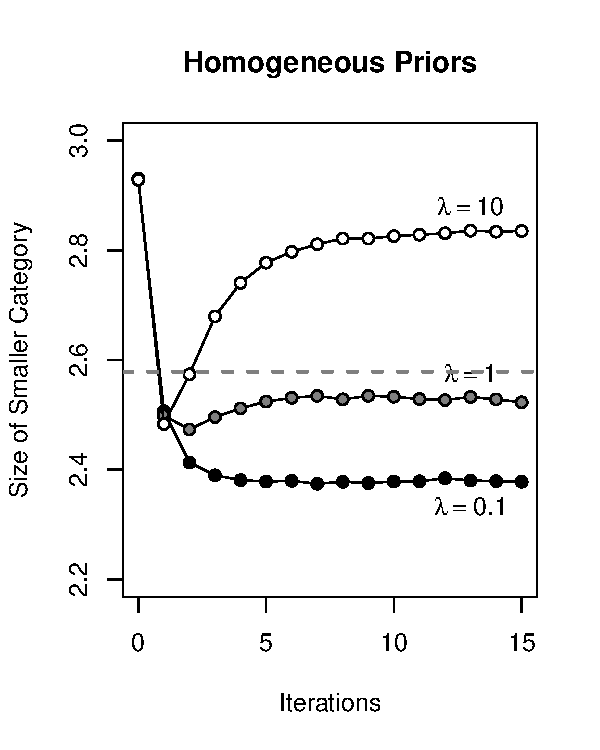
\includegraphics[width=6cm]{catsizepure.pdf} 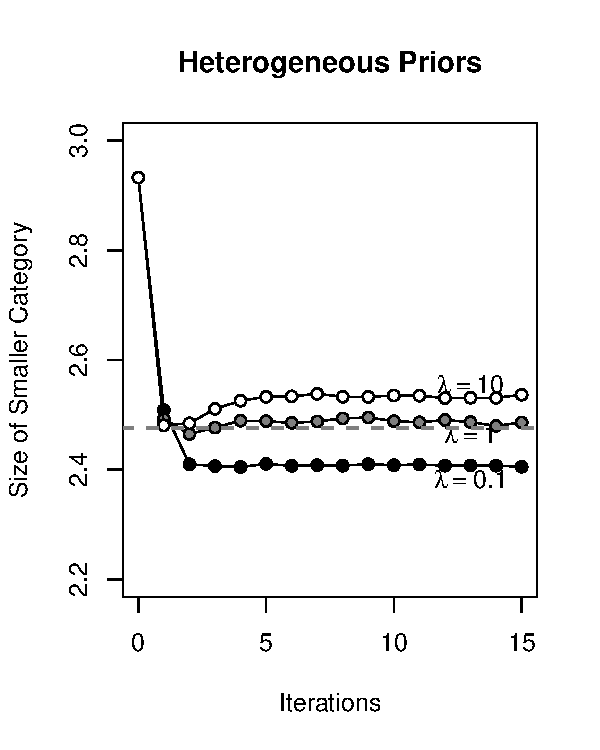
\includegraphics[width=6cm]{catsizemixed.pdf}
%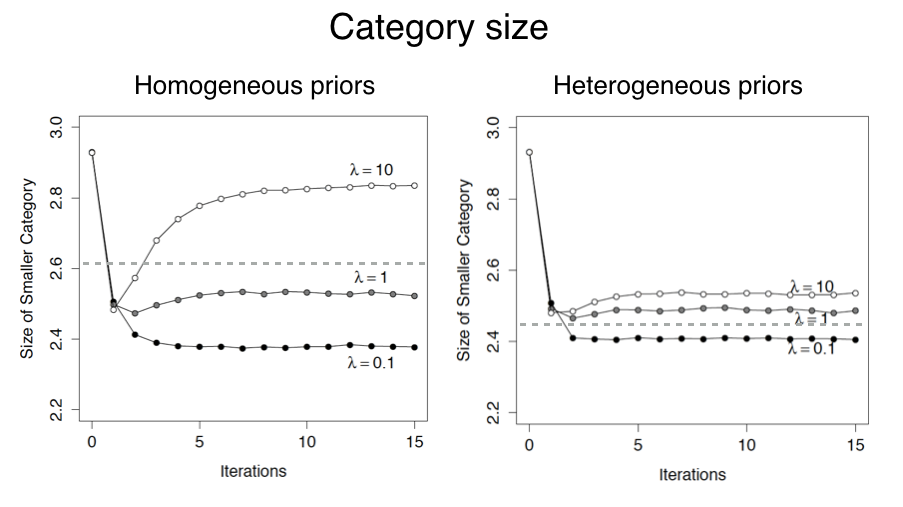
\includegraphics[width=12cm]{catsizeall.png}
\end{tabular}
\caption{\small{Category size: Performance of iterated learning chains in a supervised learning categorization task. The $y$ axis shows the preference for skewed categories, as reflected in the number of items in the smaller category: 1 indicates the maximum degree of skew, while 4 means both categories are equally sized. {\bf Left panel}: Relative size of the categories assuming all participants share the same prior ($\lambda$). Here there are three chains each reflecting one of three $\lambda$ values. As $\lambda$ grows higher, iterated learning produces more equally-sized categories. The gray dotted line reflects the average of the three chains. {\bf Right panel}: When there are individual differences within participants, the overall average category skew in the iterated learning chain is larger (i.e., the size of the smallest category is smaller) than the average of the three participant types taken separately (gray dotted line in left panel). As before, this is because the behavior of learners with larger $\lambda$ is pulled more towards the behavior of learners with smaller $\lambda$, rather than vice-versa. All results reflect 100,000 simulations for each separate chain.}}
\label{catsize}
\end{center}
\end{figure}

Categorization is a complex enough task that even when stimuli vary on only a single dimension there are many different ways of describing the inductive biases that a learner possesses. A preference for coherent categories is one kind of bias that a learner might express, but one might be just as interested in exploring the extent to which learners prefer categories to be of similar size. For instance, the category structures AAAABBBB and ABABABAB have different degrees of coherence, but both schemes divide the exemplars into two equal-sized categories. By contrast, the categories ABBBBBBB and AAAABBBB are equally coherent, but the first one divides the exemplars in a 7-1 split and the second uses a 4-4 split. A preference for any of these is not built into the GCM directly, but an effective preference falls naturally out of the model as a byproduct of variation in $\lambda$. We can operationalize this by counting how many exemplars are assigned to the smaller category, yielding a measure that produces value 1 when category sizes are most uneven and value 4 when they are exactly even. 

Figure~\ref{catsize} shows the category size measures for the three separate homogeneous chains (left) and the single heterogeneous chain (right) run previously. The homogeneous chains reveal that the GCM is biased to prefer unevenly sized categories. However, this bias is weak when the model generalizes narrowly ($\lambda=10$), and large when the model generalizes widely ($\lambda=0.1$). Unfortunately, almost none of this differentiation is evident when we look at the heterogeneous chains: the overall average is substantially different from when the three learner types were taken separately, and there are almost no individual differences to be found, with all three learner types producing similar responses. In this instance, mixing learners with different biases into the iterated learning has almost completely erased their differences. 

The explanation for why this occurs is the same as before. Here, the bias for unevenly-sized categories is the stronger one. This means that a learner with a stronger bias for unevenness (with $\lambda=0.1$) that was given equally-sized categories as input would tend to create output that was more uneven. Critically, however, a learner with less of a bias for unevenness (with $\lambda=1$) also has less strong of a preference in general. They would therefore tend to preserve any unevenness they are given. The end result is that unevenly-sized categories are much more common than a simple averaging of the preferences of the learners would suggest. As in the previous two case studies, it is the asymmetrical response between learners with different biases that is critical.

\subsection{Case study 4: A systematic exploration}

Each of the three case studies presents an example in which heterogeneity among learners introduces systematic biases to an iterated learning chain. At a qualitative level we see two distinct effects: (a) iterated learning tends to erase individual differences and (b) learners that have strong inductive biases have greater influence on the chain. In this section we present a more systematic exploration of the factors that shape these two effects. 

The scenario we consider is  deliberately generic. In it, each learner is asked to produce one or more continuous-valued judgments $x_i$. These judgments are assumed to reflect some latent belief $b_i$ possessed by the learner plus some normally distributed error (assumed to have mean 0 and standard deviation 1). Before receiving any input, the learner is uncertain what to believe about the task, captured by the prior $b_i \sim \mbox{Normal}(\mu_i, \sigma_i)$. When shown the judgments made by the previous learner $x_{i-1}$ the learner arrives at the posterior distribution $P(b_i|x_{i-1})$, samples their belief $b_i$ from this distribution, and then generates their own judgment(s) $x_i$ accordingly.\footnote{As this is a conjugate prior, the posterior distribution $P(b_i | x_{i-1})$ is also a normal distribution, with mean $(\sigma_0^{-2} + n\sigma^{-2})^{-1}$ and variance $(\sigma_0^{-2} + n\sigma^{-2})^{-1}(\mu \sigma_0^{-2} + (\sum x_{i-1}) \sigma^{-2})$, where $\sigma_0^{2}=1$ is the variance of the measurement error.} This model allows a clear separation between the ``value'' of the learner's inductive bias (i.e.,  $\mu$) and the ``strength'' of that inductive bias (i.e., $1/\sigma$). Using this model we consider heterogeneity in two different scenarios. 

\smallskip
\subsubsection{Discrete groups} Mirroring the set up in case studies 1 and 2, we first consider the situation where there are two qualitatively distinct groups of people in the iterated learning chain. The first group is always assumed to have the same direction of prior bias (given by setting $\mu_1=0$) and strength of prior bias (given by $\sigma_1=1$). We then systematically vary the properties of the second group with the goal of fully characterizing how the stationary distribution of the iterated learning chain depends on a variety of factors. These factors include: the strength of the bias of group two relative to group one (manipulated by varying $\sigma_2$); the dissimilarity in beliefs across groups (manipulated by varying $\mu_2$); the bottleneck (manipulated by varying the amount of data generated by each learner $n$); and the relative proportion $p$ of people in each of the two groups. We set default values of $\mu_2=1$, $\sigma_2=1/3$, $n=3$, and $p=0.5$, and then varied each parameter separately, running 5000 iterated learning chains at every parameter value, reading off the state of the chain after 50 iterations. We recorded the actual hypothesis (i.e., the latent belief $b_i$) sampled by each simulated participant, and compared the average belief elicited via iterated learning to the relevant priors. 

\begin{figure}[!h]
\begin{center}
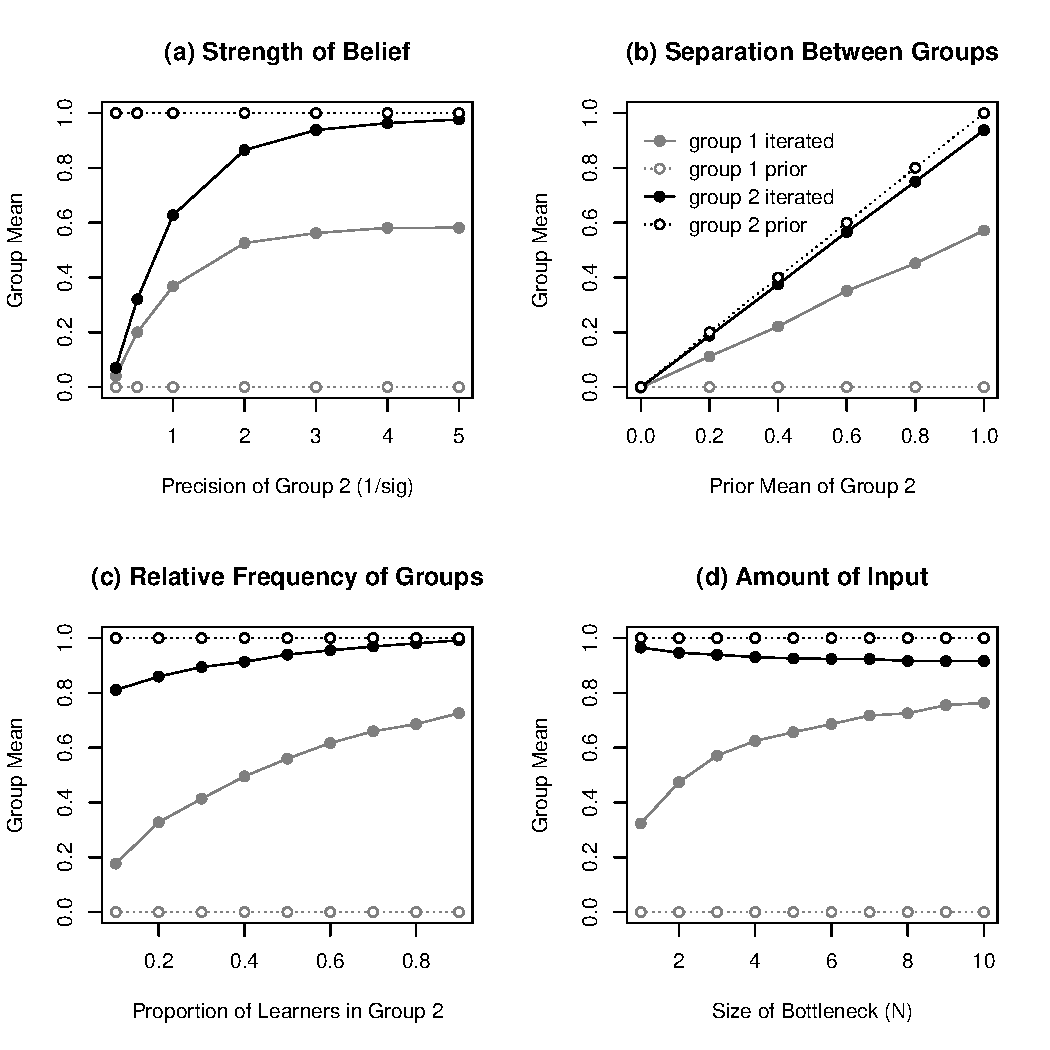
\includegraphics[width=14cm]{two-group-sim.pdf}
\caption{\small{A systematic exploration of four factors that affect the behavior of heterogeneous iterated learning chains, in situations where there are two discrete groups of participant in which group 2 is generally more strongly biased. In each panel the solid lines plot the average belief $b$ expressed by a member of each group elicited via an iterated learning chain (gray = group 1, black = group 2), and the dotted lines show the average belief that would be expected if the judgments were sampled from the relevant prior. The population shifts towards the group 2 belief as the strength of the bias in group 2 is increased (panel a), as there is more separation between groups (panel b), as group 2 makes up more proportion of the population (panel c), and as bottleneck size increases (panel d).}}
\label{fig:two-group-sim}
\end{center}
\end{figure}

As Figure~\ref{fig:two-group-sim} shows, the results of the simulation are mostly as one might predict. When the strength of the inductive bias in group 2 is increased (left to right in panel a), all learners in the chain express beliefs that are closer to the group 2 bias. Increasing the separation between the groups (panel b) induces a proportional change in everyone's beliefs. Increasing the proportion of people in group 2 shifts the average belief of both groups towards the group 2 bias (panel c). The most interesting finding is the effect of widening the bottleneck (panel d). As one would expect, the more information exchanged between learners, the stronger the homogenizing effect (the curves converge). However, the effect is asymmetric: the strong bias learners (group 2) are only very weakly affected, whereas the weak bias learners (group 1) are greatly affected. The wider the bottleneck, the more learners with strong biases dominate over learners with weak biases. 



\smallskip
\subsubsection{Continuous variation} Extending the set up in case study 3, we also consider a situation in which every learner in the chain has their own idiosyncratic mean $\mu_i$ and standard deviation $\sigma_i$, sampled randomly from some population distribution. For the population distribution over learner bias $\mu_i$ we consider two possibilities, a {\it symmetric} distribution in which the learner biases are normally distributed around 0, and an {\it asymmetric} distribution in which the biases have mean 0 but are positively skewed. For simplicity, we assume that the strength of belief $\sigma_i$ is a fixed function of the value of the bias $\mu_i$, and consider three possibilities for how the strength and value of an inductive bias might be related. In the {\it equal strength} condition all learners have the same strength of belief $\sigma$, in the {\it confident extremes} condition the learners with the most extreme biases also have the strongest confidence, and in the {\it confident center} condition the learners with the most moderate beliefs have the greatest confidence. We considered all six possible combinations of these two factors, aggregating over 10000 iterated learning chains in each case. For simplicity, we assumed that only a single observation $x$ is generated by each learner in the chain, but reduced variability in responses from 1 to 0.1 to ensure that this one response would be considered informative to most learners in the chain.


\begin{figure}[p]
\begin{center}
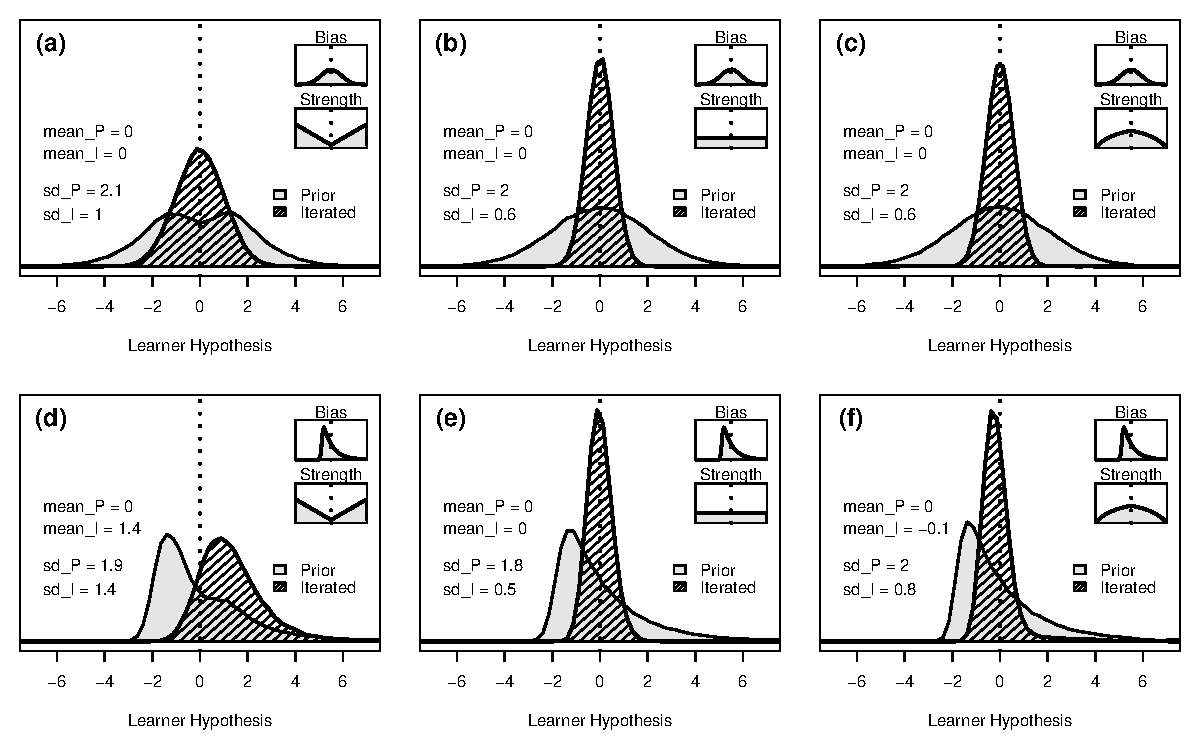
\includegraphics[width=16cm]{cont-draw-plot.pdf}
\caption{\small{Systematic exploration of the behavior of heterogeneous iterated learning chains when individual differences are continuous}. In the top row, individual differences are normally distributed (\textit{symmetric} condition), whereas in the bottom row there is a positive skew (\textit{asymmetric} condition). In the middle column, all learners have the same strength of bias no matter where their belief falls on the scale (\textit{equal strength}), whereas on the left it is the learners on the tails of the distribution that have the strongest biases (\textit{confident extremes}), and on the right the strongest biases occur in the middle of the distribution (\textit{confident center}). In each panel, the solid plots depict the marginal \textit{prior} distribution over the latent belief $b$ taken across the entire population, whereas the shaded plots show the corresponding marginal distribution over the beliefs $b$ elicited by an iterated learning procedure. The inset panels indicate which distribution condition (symmetric or asymmetric) and which bias condition (confident extremes, equal strength or confident center) is depicted, and the text annotations indicate the mean and standard deviation for each of the marginal distributions shown. It is evident that in all cases iterated learning distorts the underlying shape of population variation, and when the population is asymmetric and the extremes are more confident (panel d) it also converges to a different mean.}
\label{fig:continuous}
\end{center}
\end{figure}

The results of this simulation are shown in Figure~\ref{fig:continuous}. In every case, we observe the homogenizing effect that the iterated learning procedure has on a heterogeneous population. The standard deviation of the marginal distribution of beliefs (i.e., $b$) expressed in the iterated learning chain is always lower than the marginal prior over $b$ taken across the entire population. This effect seems to be slightly attenuated in the {\it confident extremes} condition (panels a and d), but not completely eliminated. Interestingly, in five of the six cases there are minmal effects on the {\it average} belief expressed by learners: the mean value of $b$ elicited by the iterated learning chain is the same as in the prior. However, this is not universally true. The notable exception, shown in panel d, is when the population beliefs are asymmetric and extreme beliefs are the most strongly held. When this situation arises, the confident extremists on the right hand side of the distribution have a very strong effect on the centrists (who do not hold any strong beliefs and are easily swayed). However, because the population is asymmetric there is no counterbalancing group of confident extremists on the left the distribution. Consequently, in this situation the iterated learning procedure induces a quite substantial shift in the mean expressed beliefs relative to the true priors held by learners, with the entire distribution shifting to the right. In this situation, the average belief elicited by an iterated learning procedure can be substantially different to the average belief that would be elicited if each learner sampled from their own prior.


\subsection{Summary}

Our examples all display essentially the same pattern. When all learners bring the same inductive bias to the problem, iterated learning behaves exactly in the way one might expect. Consistent with Griffiths and Kalish (\citeyear{griffiths_language_2007}), when all learners are Bayesian reasoners with identical priors and correctly specified likelihoods, the iterated learning procedure reveals those priors, while for a non-Bayesian model an analogous quantity expressing some sensible notion of preference is uncovered. However, when learners bring different biases to the problem there is no guarantee that the responses of any one participant genuinely reflects their prior biases, nor is there any guarantee that the average responses reflect the average bias in the population. 

This behavior appeared in all four of the case studies we explored. In the regularization example there were systematic distortions to the prior in both groups of participants when they were mixed into the same chain, along with systematic shifts in the mean response that overweighted those learners with the strongest biases. In the jury decision making example we were able to derive the stationary distribution of the iterated learning chain and show that it did not reveal the prior in any transparent fashion. In the categorization example we saw that the effects of heterogeneity are themselves heterogeneous: some inductive biases (like category coherence) were not strongly affected, whereas other inductive biases in the same task (like category size) were very heavily distorted by the presence of individual differences. In our final example, we see that these effects are systematic, become more severe as the information bottleneck widens, and can be observed regardless of whether individual differences are discrete or continuous.

These results are the consequence of any intergenerational information transmission process that operates where some learners hold beliefs that are more extreme than others. The central reason for this result is that the biases and knowledge possessed by one learner influences the learning and output of the next. Therefore, if different learners respond asymmetrically to the output, then their pooled output will not be reflective just of their own biases. Rather, it will be some amalgam of the two that weights the most biased learners the most heavily. Critically, it is not necessarily reflective of the ``pure'' inductive biases possessed by anyone, either individually or in aggregate. 

In the final section we empirically demonstrate that this effect has implications for using iterated learning experiments to infer people's biases. We present an experiment in which we constructed iterated learning chains from the responses of two distinct populations of human learners. As our simulations predicted, the output of the chains was heavily shaped by those with the more extreme biases. The result is a chain that does not reflect the average of all of the learners and also distorts the responses of each learner type taken separately.


\section{Experiment}

\subsection{Overview}

The purpose of this experiment is to explore, using real human data, whether chains constructed out of heterogeneous populations fail to converge to the prior as our simulations would predict. Our procedure was inspired by the ``ask a friend'' option used in a number of game shows, and loosely mirrors the structure of the jury decision making scenario in our second case study. In the experimental scenario, participants are asked to answer a question about which they (may) have some preexisting knowledge. However, they are also given a recommendation from another person that they can rely upon if they choose. The learner's task is to integrate their prior knowledge with the new information to arrive at a decision. Since the intent of the study is to capture the biases and responses of people who we already know have very different priors, we chose to ask questions about Australian politics to two groups of people: Australians and Americans. Similar to \textcite{ferdinandetal13}, rather than running iterated learning experiments directly we then constructed iterated learning chains from those biases and priors, systematically manipulating the proportion of Americans and Australians in each chain. This procedure constructs chains that are indistinguishable from those gathered through direct experimentation, because the response any participant depends only on the information they are prompted with (the advice, in our experiment), and not on the order in which those events occurred. Our question was whether the output of the iterated learning chains with mixed participants matched the separately-estimated priors. 

\subsection{The scenario}

In our experiments, people were asked to answer a question about Australian politics based on a combination of their own knowledge and the input of one other person, which they can weight as they choose. Formally the problem is similar to the jury decision making problem, and can be modeled in a similar way. Each learner is assumed to have some subjective beliefs from which a prior distribution over the outcomes $P(o)$ can be constructed: Americans may recognize the names of one or two Australian politicians only, while Australians may have much more nuanced knowledge. They also have some confidence in their own beliefs relative to the advisor: most Americans may realize that they don't know much about Australian politics, while Australians may differ more widely in their confidence. 

To provide a simple model for this task, we consider a modest extension of the Bayesian model used to specify the {\sc sheep} and {\sc goat} learners in our second case study. As before, the learner assigns some degree of reliability to the advisor, and the extent of the learner's belief revision will depend on this reliability. Specifically, the model that the advisor provides the correct response with probability $r$ and chooses randomly among the remaining $n-1$ options with probability $1-r$. The larger the value of $r$, the more likely the participant is to rely on the advisor. In this model, the posterior probability $P(o|a)$, over outcomes $o$ given advice $a$, is
$$
P(o|a) = \frac{P(a|o) P(o)}{\sum_{o^\prime} P(a|o^\prime) P(o^\prime)}
$$
where the likelihood $P(a|o)$ equals $r$ if $a=o$ and $(1-r)/(n-1)$ otherwise. Figure~\ref{advice} illustrates the role of confidence in the advisor for a situation with four different options (A-D). If a learner with the prior beliefs about options A-D depicted in the left hand panel is not very confident in the advisor, their responses will more closely match their prior beliefs, as in the middle panel. If, on the other hand, they are confident that the advice is correct they are likely to follow it, as in the right panel. 

\begin{figure}[t]
\begin{center}
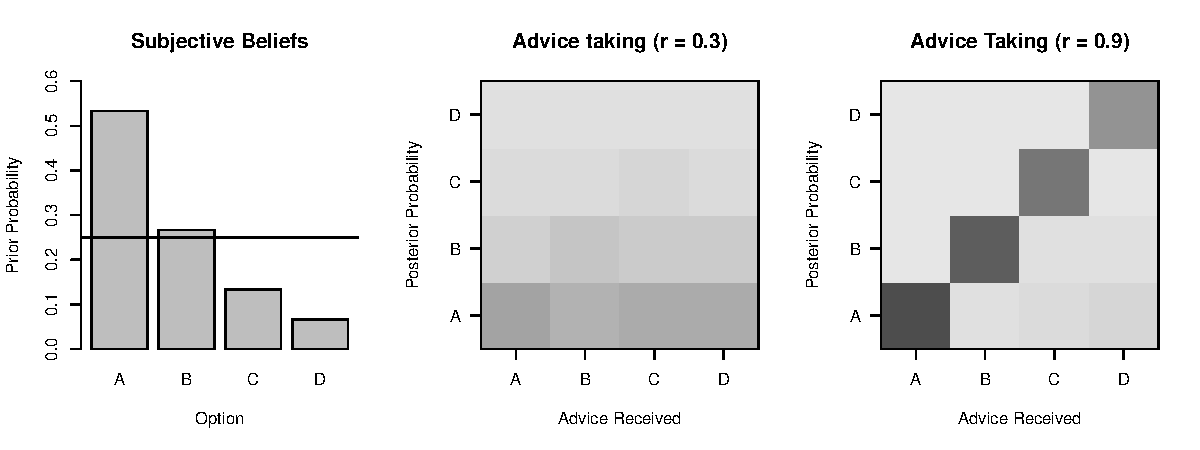
\includegraphics[width=13cm]{advice.pdf}
\caption{\small{A simple Bayesian model for the advice taking problem. The left panel plots a subjective probability distribution over options A-D -- the prior. The middle panel plots the posterior probability over these options conditional on each possible piece of advice (darker = more probable), for a learner who believes that the advisor is correct with probability 0.3 (only slightly above chance) and therefore relies primarily on their own beliefs -- roughly analogous to the {\sc goats} in case study 2. The right panel plots the same results for a situation in which the learner believes the advisor is correct with probability 0.9, more or less consistent with the {\sc sheep} jurors in case study 2.}}
\label{advice}
\end{center}
\end{figure}

As with the previous examples, the iterated learning method implies that if everyone shares the same prior $P(o)$ and samples responses from the posterior $P(o|a)$, the long run behavior of an iterated learning chain should reflect the prior. %If each participant's response is used as advice for the next person in the chain, we would expect the final distribution of responses to be $P(o)$. 
% AP: this is incorrect, isn't it? if everyone relies on everyone else for advice, it's totally distorting the priors and double-counting things, as in case study 2.
However, the analysis in this paper suggests that when individual differences are present, we should not expect the result to adequately reflect individual priors. Specifically, we should expect to see systematic distortions in which the responses of individual subjects are shrunk towards the beliefs of other participants, with the participants who are more like the {\sc goats} (i.e., unwilling to change their beliefs based on the previous person in the chain) having a stronger influence on the overall chain. 

In order to investigate the extent to which this might occur in practice, our experiment is designed to elicit priors and responses in two different ways. In the {\sc direct elicitation} condition we simply ask people to report their priors $P(o)$; this allows us to produce plots similar to the left panel of Figure~\ref{advice}. In the {\sc advice taking} condition we present participants with a specific piece of advice and ask them to make a decision; this allows us to produce a ``transition matrix'' analogous to those shown in the middle and right panels of Figure~\ref{advice}. This approach to studying cultural transmission was previously used by \textcite{ferdinandetal13}. By recruiting participants with different levels of knowledge about a topic, we can control the extent to which individual differences are present in the sample. We then use this to investigate the behavior of iterated learning chains in practice.

\subsection{Method}

\subsubsection{Participants}

The experiment collected data from two populations expected to possess different inductive biases, workers on Amazon Mechanical Turk (MTurk) and undergraduate students at UNSW in Sydney, Australia. MTurk workers were paid US\$0.85 for 5 minutes, whereas the UNSW students were a self-selected sample who participated for course credit. Ten MTurk participants were excluded as they were not located in the US. 

Two versions of the task were presented. A total of 320 participants (196 on MTurk, 124 at UNSW) completed the {\sc advice taking} task and an additional 80 participants (38 MTurk, 42 UNSW) completed the {\sc direct elicitation task}. Demographics for the {\sc advice taking} task were as follows. The MTurk sample was 64\% male, ranging in age from 18 to 67 (mean: 36.6), while the UNSW sample was 23\% male, ranging in age from 17 to 49 (mean: 19.6). In the {\sc direct elicitation task}, the MTurk sample was 76\% male, ranging in age from 18 to 67 (mean: 33.7). The UNSW sample was 14\% male, 2\% other, and the rest were female, with an age range of 17 to 34 (mean: 18.9). For simplicity, we henceforth refer to the MTurk sample as Americans and the UNSW sample as Australians.

\bigskip
\subsubsection{Procedure: advice taking}

The task was completed via a Qualtrics survey with two items. One pertained to the NFL Draft and is not included here for space reasons.\footnote{Its results are consistent with the rest of the paper, demonstrating that an iterated learning chain composed of people with distinct priors does not converge to an average of those priors, and systematically distorts the behavior of the individuals in the chain.} The other item pertained to the 2016 Australian election, which had not occurred at the time of the experiment. It asked people to guess who would be the Australian Prime Minister after the election, presenting four options to choose from: Malcolm Turnbull, Bill Shorten, John Howard and Gordon Brown. Two of the options were high-familiarity lures: as retired former Prime Ministers of Australia and the UK respectively, neither John Howard nor Gordon Brown were available as candidates in the election. As the leaders of the two major Australian political parties, Malcolm Turnbull and Bill Shorten were the only two plausible choices. These facts would be obvious to the vast majority of Australians, but represent obscure knowledge for most American citizens. 


The questionnaire was designed in a format that provides input from other agents. People were presented with ``advice'' from a friend recommending that they select one of the four options (chosen randomly from the four possibilities). The advisor was described as very knowledgeable about the subject matter, as somebody who follows Australian politics extremely closely. However, they were also implied to be potentially unreliable (because they have been consuming alcohol). Presenting the advice in this format was deliberate, as it allows a genuinely knowledgeable participant to explain why their supposedly knowledgeable friend is giving foolish advice (e.g., they're drunk and so are predicting that John Howard will make a spectacular return to Australian politics). It also allows the freedom for a participant to rely on the advice (e.g., thinking, okay, they've been drinking but they probably still know the answer). The exact wording of the question was as follows:

\begin{quotation}
Imagine that you are at your local bar with some friends. After several drinks, the topic of conversation turns to politics. You are asked for your opinion on which of the following politicians will win the next Australian Federal Election. 

One of your close friends recommends that you say [insert option]. You know that they follow Australian politics quite closely and know a lot about it; on the other hand, they have just had several alcoholic drinks. In light of their recommendation, who do you think will win the election?
\end{quotation}


\bigskip
\subsubsection{Procedure: Direct elicitation}

The direct elicitation task used the same question, but adopted a much simpler procedure. People were simply asked to assign probabilities to the four alternatives (expressed as percentages), where the numbers were constrained to add up to 100\%, using a sliding bar interface.

\subsection{Results}

\begin{figure}[t]
\begin{center}
%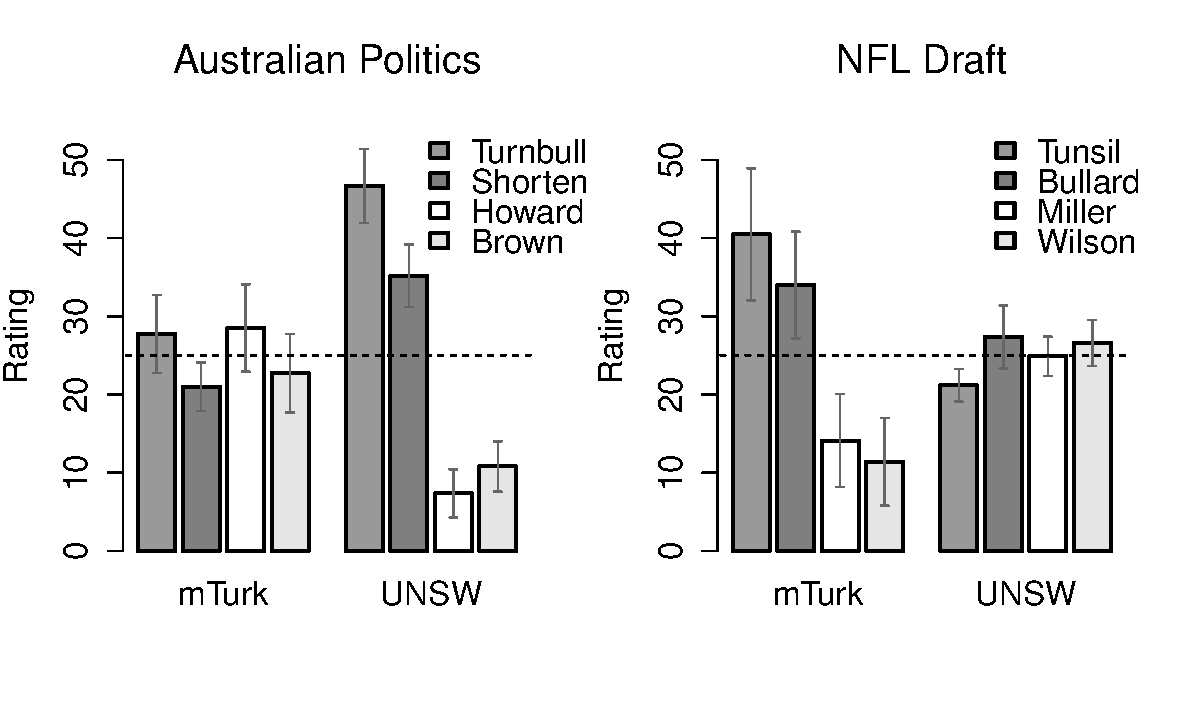
\includegraphics[width=11cm]{priors.pdf}
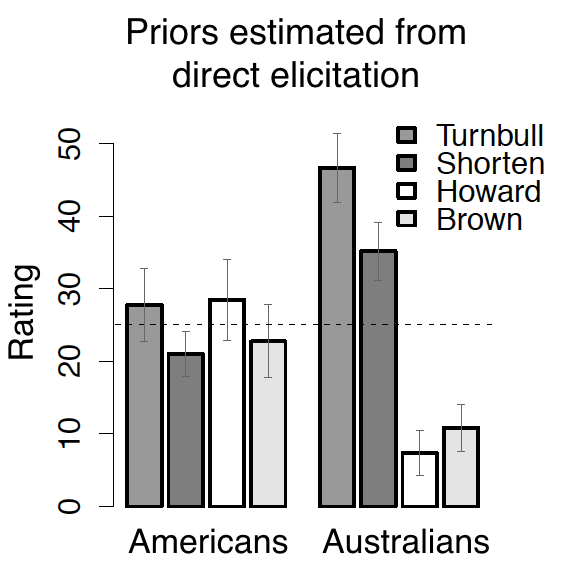
\includegraphics[width=7cm]{priorsozelection.png}
\caption{\small{Average reported prior probabilities in the {\sc direct elicitation} task. Most Australian participants correctly recognized that Turnbull and Shorten were the only legitimate candidates, whereas the American participants rated all four options about equally, suggesting that they had no relevant knowledge about the topic. }}
\label{direct}
\end{center}
\end{figure}


The results from the direct elicitation task are plotted in Figure~\ref{direct} and confirm our hypothesis about the different prior beliefs across the two participant pools. The Australian participants correctly recognized that John Howard and Gordon Brown were not legitimate candidates for Australian Prime Minister, giving most probability to Malcolm Turnbull (47\%) and Bill Shorten (35\%). In contrast, the American participant responses were more or less uniform across Turnbull (28\%), Shorten (21\%), Howard (29\%) and Brown (23\%). 

\begin{figure}[t]
\begin{center}
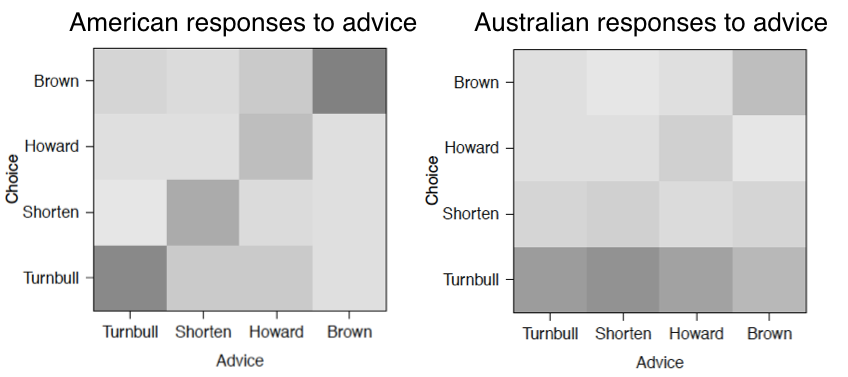
\includegraphics[width=12cm]{transitionsozelection.png}
\caption{\small{Empirical transition matrices estimated from the {\sc advice taking} task. The advice is shown on the $x$ axis, while the choice of the participant is on the $y$ axis. Americans (left panel) tended to follow the advice they were given about the Australian election, as reflected in the darker colors on the diagonal. By contrast, Australians (right panel) were likely to pick Malcolm Turnbull regardless of what they were advised to do. This reflects differences in confidence about their prior beliefs, which affects the degree to which they are influenced by their input.}}
\label{transitionsozelection}
\end{center}
\end{figure}

In the {\sc advice taking} scenario, the results are also fairly predictable. As illustrated in Figure~\ref{transitionsozelection}, when participants are not knowledgeable about the topic they follow the advice they are given, but tend not to if they know about the topic. Most (60\%) American participants followed their advisor but the Australian participants tended to choose Turnbull (58\% of responses) regardless of the advice given. Note the similarities between Figure~\ref{transitionsozelection} and \ref{advice}: in this context the American participants gave responses similar to the {\sc sheep} in case study 2 where the Australian participants behaved in a fashion more akin to the {\sc goats}, which has implications for their relative ability to influence an iterated learning chain.


\subsection{Simulated iterated learning chains}

\begin{figure}[t]
\begin{center}
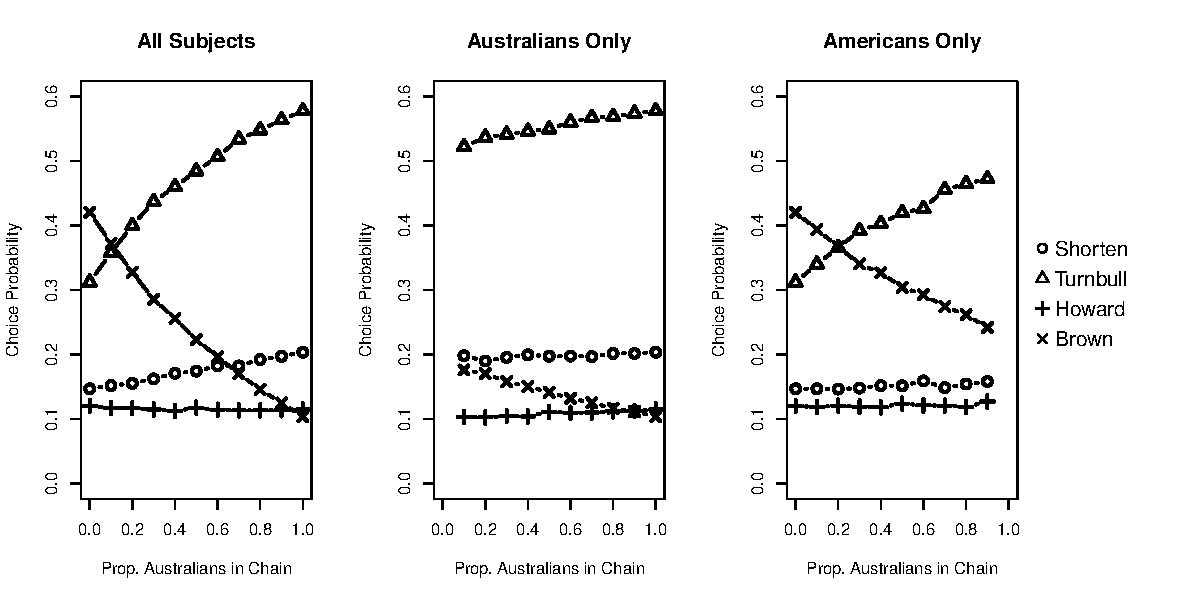
\includegraphics[width=15cm]{chainPol.pdf}
\caption{\small{Long run behavior of simulated iterated learning chains, plotted as a function of the probability $\theta$ of updating the chain with an Australian participant ($x$ axis). The $y$ axis reflects the proportion of each of the four possible candidates, which in a typical iterated learning analysis would be assumed to reflect people's priors.  {\bf Left panel}: Response proportions from each chain as a whole. As more Australians are included in the chain, the probability assigned to Turnbull increases. Strikingly, it is necessary for the chain to include only a small proportion of Australians (between 10\% and 20\%) for Turnbull to become the modal response. The reason for this is shown when we break down responses by participant group. {\bf Middle panel}. Responses from only the Australians in each chain reveal relatively little change as more Australians are included: the Australian participants are not strongly influenced by the input they are given. {\bf Right panel}. Responses from only the Americans in the chain show that they are highly distorted by the presence of Australians, appearing to select Turnbull by a wide margin even though Americans' actual priors were uniform over all four options.}}
\label{chainPol}
\end{center}
\end{figure}


The data from the {\sc advice taking} task allow us to examine how iterated learning chains behave in the presence of systematic differences among participants. The experiment produces a transition matrix of exactly the sort that iterated learning chains require -- one that gives the probability of each possible response given each possible input, as in Figure~\ref{transitionsozelection}. Using this matrix, we can investigate what an iterated learning chain involving different combinations of these participants would look like. A participant is initially selected at random and their response (e.g., Turnbull) is ``fed'' to the next simulated participant by sampling a participant randomly with replacement from those participants who were given ``Turnbull'' as their advice. 

This method makes it straightforward to simulate chains with different proportions of each of the two populations (Americans or Australians). At each step, a participant is chosen from either population with some fixed probability $\theta$ and their response is selected based on the transition matrix of that population. By systematically varying $\theta$ in different chains, we can explore the effect of different levels of heterogeneity, from completely homogeneous (with chains composed entirely of Americans or entirely of Australians) to maximally heterogeneous (with a chain composed of half Americans and half Australians). Given our previous analysis as well as the observed priors and transition matrices, we expect that mixing the two populations together in a single chain should be expected to systematically distort the chain away from the performance of either group individually, or what one would get by simply averaging their priors. Because of their much stronger tendency to follow the advice they are given, American participants should exert less influence on the chain as a whole, and should be more willing to adjust their responses to mimic Australian participants than vice versa. 

To evaluate this, we simulated iterated learning chains using the procedure outlined above, systematically varying the probability of selecting an Australian participant.\footnote{Our simulations use 100,000 iterations and a burn-in of 1,000 iterations, producing very smooth curves. However, because the chains sample with replacement from a set of 320 participants, these curves are still subject to sampling error.} The results, shown in Figure~\ref{chainPol}, are as expected. The left panel shows the behavior of the entire chain as a function of the proportion of Australian participants. As more Australians are included, the probability assigned to Turnbull increases far more than a simple weighted average over prior beliefs would suggest it should. In fact, the chain need only include a small proportion of Australians (about 10-20\%) for Turnbull to be the modal response. 

To understand why this happens, we can separately analyze the responses of Australian (middle panel) and American (right panel) participants in the chains. When the chain consists entirely of Americans (left-hand side of both panels), there are no Australian responses and the American workers therefore produce answers that are consistent with the transition matrix plotted in the top left panel of Figure~\ref{transitionsozelection}: 42\% of responses are Brown, followed by 30\% Turnbull. However, as we start to introduce more Australians responses into the chain, the distribution of responses produced by {\it Americans} changes systematically, because the biases of the Australians affect the Americans via the input they receive. The more Australians in the chain, the more the Americans favor Turnbull. In the extreme case where the chain is 90\% Australians and only 10\% Americans, those Americans are producing responses that are 47\% Turnbull and only 24\% Brown. Of critical importance, however, the effect is not symmetric. Because the Australians are much more confident in their knowledge than the Americans, the Australians reduce the degree to which they choose Turnbull far less than the Americans increase theirs. Accordingly, the prior beliefs held by Australian participants exert a disproportionate influence on the chain as a whole.\footnote{More precisely (since we simulated the chains by sampling responses in the empirical data) it is the transition probabilities in Figure 15 that exert this influence, which are presumably shaped by the prior beliefs held by Australian and American participants. The precise relationship between the two depends on how responses are generated. For instance, if participants were using MAP estimation rather than sampling from the posterior, then the homogeneous chains (i.e., all Australian or all American) will reflect an exaggerated version of the participant priors, as shown in Figure 5.}

\subsection{Discussion}

The pattern of results is intuitive and in some respects unsurprising: the inference problem pertains to Australian politics, the Australian participants brought considerable prior knowledge into the task, and their responses were almost entirely unaffected by the advice they were given. In contrast the American participants entered the task with very little prior knowledge, and relied almost entirely on the advisor. This naturally created a ``{\sc sheep} versus {\sc goats}'' scenario when we use the data to construct an iterated learning chaining. Only a very small number of Australian participants need to be injected into the chain to produce very substantial changes in the responses produced by the American participants. Arguably this is very sensible behavior, with the American participants wisely deferring to the better knowledge that the Australian participants had. However, it does very strongly imply that the responses produced by the American participants in the heterogeneous chain do not in any meaningful sense reflect their prior knowledge about {\it Australian politics}. Without any Australian influence, the American participants produce iterated learning chains that don't converge to anything sensible (the apparent bias for Gordon Brown possibly reflects name recognition based on UK politics), yet in a chain that consists of an equal mixture of Australian and American participants those same participants would produce responses that look considerably more knowledgeable. In essence, the long run behavior of our mixed iterated learning chain does not reflect a ``shared'' prior, nor does it represent a ``weighted average'' of individual priors -- rather, it is disproportionately influenced by those individuals with the strongest biases. 



\section{General discussion}

Our work represents a natural extension to the  results presented by \textcite{griffiths_language_2007}. In their original work, iterated learning with Bayesian agents was shown to converge to the prior if those agents all share the same prior and likelihood. However, when these assumptions do not hold, there can be systematic departures from this pattern. Implications of this are briefly discussed below.

\subsection{How widely do these results hold?}

The general pattern we observe is that when individual differences exist, iterated learning chains tend to have a homogenizing effect which minimises these differences and overweights the contributions of those learners with the strongest biases. How widely do these results hold? Based on our simulations, the homogenizing effect appears to be especially pervasive, appearing in every one of our case studies, including situations involving non-Bayesian models. However, in some instances this homogenizing effect is modest, particularly if the information bottleneck is narrow. This pattern is consistent with earlier work by Ferdinand and Zuidema (\citeyear{ferdinand2009thomas,ferdinand2008language}) who also found in a more restricted setting that the size of the bottleneck matters considerably for heterogeneous iterated learning chains.

With regards to the disproportionate influence of ``extremists'', a little more care is required. As far as we can tell, learners with extreme biases always have a stronger influence on other learners (we found this in every one of our examples). However, this does not always lead to a systematic shift in the overall distribution of responses. Perhaps the clearest illustration of this was the finding shown in Figure~\ref{fig:continuous}: in the continuous setting, the iterated learning chain only produces a shift in the mean of the response distribution when there are learners with extreme and strongly held biases {\it and} there are no counterbalancing extremists on the other side of the distribution to counteract their influence. This probably explains why \textcite{ferdinand2008language,ferdinand2009thomas} did not find evidence of systematic distortion despite considering heterogeneous iterated learning chains. Their heterogeneous agents happened to have equally strong prior biases, thus counterbalancing each other.

%: in both of their groups, the learner assigns 60\% probability to the most likely hypothesis and spreads the remaining belief evenly across the other options. In our simulations we found analogous results: if all learners have equally strong biases, there is no overall distortion to the mean response. 

%In the case of \textcite{burkettgriffiths10}, the heterogeneity occurs because there are multiple teachers in the chain; however, agents' priors are well-calibrated, thus ensuring convergence to the prior.

\subsection{Broader implications}

The paradigm of iterated learning leads a bit of a  double life within the psychological literature. As a result, the implications of our work dependon the context in which it is to be applied. As a theoretical tool, the underlying dynamics of iterated learning chains provide valuable insights into how information is transmitted between individuals or generations. %In this context the convergence behavior of the chain is important, but it is not essential that the chain converge to {\it the prior} in any meaningful sense. 
Our results are important because, unlike other work exploring circumstances in which iterated learning distorts the prior (e.g., Kirby et al., 2007), we find that this distortion is hard to precisely characterize and also means that some individuals have more influence than others. Who those individuals are and exactly what their influence is may vary considerably depending on the domain the learning situation.

%Rather, our results make an important point about cultural evolution when learners bring different prior biases. We show that learners with the strongest biases exert the greatest influence on the chain. This is consistent with the idea that some subpopulations, like young children, might exert a stronger influence on linguistic evolution than others. 

Similarly, we found that learners with the most confidence in their own beliefs will be less influenced by others and their beliefs will also exert a disproportionate influence on others. As is sometimes noted \parencite[e.g.,][]{russo_managing_1992}, the ability to influence others in this fashion provides a motivation to express confidence, and in turn provides a partial explanation for the pervasive overconfidence effect \parencite[e.g.,][]{lichtenstein_calibration_1977} in human judgment. If the goal is to have cultural influence rather than be correct, strong biases are better than weak ones.

However, our simulation results also suggest a natural and slightly counterintuitive extension of this theory: that individual underconfidence can produce collective overconfidence. In the jury decision-making scenario, the behavior of a chain of {\sc sheep}-like jurors produced perverse outcomes even though all jurors were Bayesian reasoners sharing the same priors. While each individual juror was underconfident -- in the sense of underweighting the relative importance of their own beliefs relative to the input of others -- the stationary distribution of a chain of such learners ended up {\it overconfident}, insofar as it exaggerated the prior beliefs of all learners. This effect is strikingly reminiscent of the groupthink phenomenon \parencite{janis1982groupthink,esser_alive_1998}. Our results suggest that Bayesian reasoners are no more immune to such effects than any other kind of learner, in the (very likely) event that the learner does not have perfectly calibrated confidence in their own beliefs. 

\subsection{Iterated learning as an elicitation tool}

On the methodological side, iterated learning has often been used as a tool for exploring the inductive biases of individuals. Based on formal results suggesting that the stationary distribution of an iterated learning chain is the prior, researchers in cognitive science have sometimes used these designs as a form of elicitation task, in which the (between-subject) distribution of responses is taken to be reflective of some (within-subject) latent mental representation of the world. Our results suggest that such conclusions may be unwarranted whenever individual differences are present. When people bring different priors to a task, there is no inherent reason to think that the stationary distribution of an iterated learning chain bears any meaningful relationship to those priors. The distortions are systematic in the sense that stronger biases lead to disproportionate influence, while simultaneously being difficult to predict in the sense that one cannot specify with any precision in what way that disproportionate influence is realized. 

This lack of predictability is especially troublesome from a methodological point of view. In our third case study, it was not at all obvious to us that heterogeneity among category learners would produce a very large distortion of ``category size'' biases but almost no distortion to the bias for ``coherent'' categories. Indeed, without some {\it other} method for checking that one's participants all share the same beliefs and that those beliefs are not mis-calibrated as in {\sc sheep} jurors -- as well as some tool for verifying how sensitive a particular bias is to distortion via the iterated learning methodology -- it is hard to see how any researcher can be confident that an iterated learning experiment has revealed a ``real'' inductive bias. On this front, we are a little more skeptical of the utility of iterated learning methods for exploring individual inductive biases.\footnote{Another methodological possibility might be to use iterated learning experiments as a tool for inferring the bias parameters of relevant cognitive models -- that is, using the input-output data pairs produced by the experiments in order to fit models. Our research here is agnostic about the utility of this method, although it represents an interesting angle for future work.}


\subsection{What are the biases that iterated learning reveals?}

Our results raise a question about what precisely constitutes an ``inductive bias''. When Bayesian reasoners are involved, the usual way of characterizing an inductive bias is through the prior distribution that a learner imposes over a set of hypotheses. As such, it is typically assumed that an iterated learning chain reveals the prior \parencite{griffiths_language_2007}. Our main result in this paper has argued that this is not true when learners have different biases. However, consistent with \textcite{smith2009iterated} we also find that iterated learning can fail to reveal the prior even when all learners are Bayesians with a shared prior. In the juror scenario, a homogeneous chain of Bayesian {\sc sheep} produced behavior that substantially misrepresents their priors. This occurs because the {\sc sheep} jurors applied the wrong likelihood function and overweighted the evidentiary value of other jurors' opinions. The fact that this miscalibration has an impact on the stationary distribution of an iterated learning chain is revealing: even with Bayesian reasoners, the ``inductive bias'' revealed by an iterated learning is not a transparent reflection of the prior distribution, but is instead a product of both the prior distribution and the likelihood. This should not be surprising. In real life, one's biases do not solely consist of the beliefs one has about the world (priors): one's willingness to have those beliefs changed and the manner in which those changes occur (likelihoods) are also a form of bias. As our results illustrate, the likelihood can shape the behavior of an iterated learning chain just as much as the priors. 

An intriguing generalization of this issue emerges when we consider the question at the population level. What inductive biases does a {\it population} of learners possess? Like most researchers in this area, we have adopted the simplest view and assumed that the population prior corresponds to the average of individual priors. Yet, in many real world situations, it might be more sensible to weight the knowledgeable or certain people more: after all, no one person retains all of the cultural knowledge of an entire population. In our experiment, for example, American participants in a heterogeneous iterated learning design were able produce more accurate responses than they would have done in a homogeneous chain, precisely because they relied on the stronger inductive biases of Australian participants. From this perspective, it might be more natural to describe the population prior in a fashion that weights highly confident individuals most heavily. Our simulations in the first case study suggest that iterated learning chains do not converge to a weighted population average of this sort either, at least not in a straightforward way, but it is at this point an underexplored issue and an opportunity for future work. 

More generally, in richer social contexts, agents need to keep track of the goals of other agents and be wary of potential deception. People often express strong opinions in order to influence others, and a learner may discount extreme or very confident opinions as a result. Initial work in our lab suggests that when learners are given the ability to make inferences about who to trust and listen to, the resulting distribution still does not converge to the prior. Rather, at least much of the time, subpopulations tend to break off and form ``echo chambers'' composed of agents who only communicate within the emergent subpopulation. Precisely characterizing these dynamics is also a matter for future work.

In general, our research shows that even within very simple iterated learning chains, heterogeneity leads unpredictable convergence outcomes. When populations of learners vary, the resulting information transmission chain is disproportionately shaped by those with stronger biases. However, exactly how and to what extent it is shaped depends on a complicated interplay of diverse factors. Given the ubiquity of individual differences across nearly every domain of human cognition, understanding the effects of heterogeneity is an important part of appropriately applying iterated learning methodologically as well as understanding cultural and linguistic evolution in the world. 


\printbibliography


\end{document}
